% ****** Start of file main.tex ******
%
% This manuscript follows the APS REVTeX 4.2 sample style.  The
% documentclass options below select a two-column Physical Review A
% layout suitable for a quantum-information manuscript.
%
% TeX'ing this file requires AMS-LaTeX and REVTeX 4.2.  The standard
% compilation sequence is
%
%  1) pdflatex main.tex
%  2) bibtex main
%  3) pdflatex main.tex
%  4) pdflatex main.tex
%
\documentclass[
 reprint,
 amsmath,amssymb,
 aps,
 pra,
 floatfix,
]{revtex4-2}

\usepackage{graphicx}% Include figure files
\usepackage{dcolumn}% Align table columns on decimal point
\usepackage{bm}% bold math
\usepackage{amsmath}
\usepackage{amssymb}
\usepackage{braket}
\usepackage{hyperref}
\hypersetup{hypertexnames=false}
\usepackage{orcidlink}
\usepackage{booktabs}
\usepackage{placeins}
\usepackage{tikz}
\usetikzlibrary{arrows.meta,positioning}
\raggedbottom
\makeatletter
\setlength{\@fptop}{0pt}
\setlength{\@fpsep}{8pt plus 2fil}
\setlength{\@fpbot}{0pt plus 1fil}
\setlength{\@dblfptop}{0pt}
\setlength{\@dblfpsep}{8pt plus 2fil}
\setlength{\@dblfpbot}{0pt plus 1fil}
\makeatother

\newtheorem{theorem}{Theorem}
\newtheorem{proposition}[theorem]{Proposition}
\newtheorem{corollary}[theorem]{Corollary}
\newtheorem{definition}[theorem]{Definition}

\begin{document}

\preprint{APS/123-QED}

% The title should be concise but literal enough for database indexing.
\title{Resource-Certified Quantum-Huffman-Inspired Source Decoding with Group-Conditioned Measurements}

% Author and affiliation lines follow the REVTeX front-matter structure.
\author{
    Songyao Xue\,\orcidlink{0009-0009-5122-0963}
}
\email{Contact author: 18637229290@139.com}
\affiliation{School of Software, Luoyang Normal University, No. 6 Jiqing Road, Yibin District, Luoyang, Henan Province, 471934, China}

\author{
    Mengsi Zhang\,\orcidlink{0009-0001-6793-9093}
}
\thanks{These authors contributed equally to this work. Songyao Xue is listed first and Mengsi Zhang second.}
\affiliation{School of Artificial Intelligence, Dalian Maritime University, No. 1 Linghai Road, Ganjingzi District, Dalian City, Liaoning Province, 116026, China}

% Any explicit date may be used; \today follows the APS sample convention.
\date{\today}

\begin{abstract}
We study a finite-resource probabilistic source-decoding model inspired by quantum Huffman coding. Huffman lengths define finite-dimensional support budgets for a source-shaped nonorthogonal ensemble in a common Hilbert space. A group ancilla transfers inter-group ambiguity into orthogonal label information, leaving smaller conditional POVM tasks. Under a declared scalarized resource convention, normalized margins decide whether success gains pay for group-label and reliability overhead. A representative benchmark yields nonpositive margins under conservative overhead, while a favorable-regime sweep identifies structured sampled regions with positive margins. Feasible grouped primal bounds and fixed-length dual upper bounds certify selected finite instances, including a controlled \(M=8\) probe; larger-\(M\) rows provide PGM diagnostics. QEC and MAP supply effective-reliability and posterior-decision layers.
\end{abstract}

%\keywords{Suggested keywords}% Use showkeys class option if keyword display is desired.
\maketitle

%\tableofcontents


\section{Introduction}

Classical Huffman coding converts a nonuniform source distribution into prefix lengths $l_i$ satisfying the Kraft inequality~\cite{shannon1948mathematical,huffman1952method,cover2006elements},
\begin{equation}
    \sum_i2^{-l_i}\le 1,
    \label{eq:kraft_intro}
\end{equation}
with average length $\bar L=\sum_i p_i l_i$. A direct quantum analogue is subtle because coherent superpositions of different codeword lengths make termination and length measurement nontrivial~\cite{schumacher1995quantum,jozsa1994new,jozsa1998optimal,braunstein2000quantum,schumacher2001indeterminate,bostrom2002lossless,hayashi2002quantum,hayashi2002simple,muller2009variable}. We therefore use classical Huffman lengths as support-budget parameters in a common finite-dimensional Hilbert space and study probabilistic decoding of the resulting nonorthogonal states.

In a coherent variable-length code, a quantum source may occupy a superposition of different length sectors. A decoder that identifies a codeword boundary or a prefix termination time can reveal length information and thereby disturb the encoded state. Schumacher compression and its refinements provide asymptotic, universal, and finite-resource perspectives on quantum source coding~\cite{schumacher1995quantum,jozsa1994new,wilde2013quantum,tomamichel2013hierarchy,tomamichel2016finite}. These observations motivate a finite-resource question: can the probability structure that makes classical Huffman coding useful shape a quantum ensemble for probabilistic decoding?

Our answer is to separate ``Huffman structure'' from ``variable-length transmission.'' The length $l_i$ is treated as a support-budget parameter, so that $2^{-l_i}$ determines a relative share of a common ambient Hilbert space. High-probability symbols receive more amplitude--phase shaping freedom, while all symbol states remain embedded in the same Hilbert space for discrimination. This avoids the coherence problem of measuring length, but preserves the source-dependent geometry induced by the classical Huffman tree.

The central contribution is the combination of Huffman-induced support budgeting and group-conditioned state discrimination under an explicit resource-efficiency test. Huffman lengths determine how much support each source symbol may occupy. The induced support geometry constrains the possible state overlaps. An orthogonal group ancilla separates inter-group alternatives exactly and leaves smaller conditional POVM tasks inside each group. QEC enters through an effective logical-failure model, and MAP correction is a block-local deterministic post-processing rule. The final question is whether the success gain compensates the group-label and physical-qubit overhead.

Compared with strict variable-length quantum coding, this model avoids coherent length transmission and termination measurement. Compared with ordinary fixed-length ensemble discrimination, it uses source nonuniformity to shape the ensemble before discrimination. Reliability and grouping are evaluated through the same resource-normalized efficiency. The resulting pipeline is summarized in Fig.~\ref{fig:pipeline}. Besides the operational flow, the figure highlights the diagnostic quantities introduced here: the Huffman-induced ambiguity budget, the ambiguity transferred by the group label, and the resource margin used to certify finite-resource advantage.

This positioning also distinguishes the present paper from standard minimum-error state discrimination and its numerical optimality methods~\cite{helstrom1969quantum,helstrom1976quantum,holevo1973statistical,yuen1975optimum,belavkin1975optimum,chefles2000quantum,barnett2009quantum,bae2015quantum,jezek2002finding}. In the usual discrimination problem, the ensemble is specified first and the task is to find the optimal measurement for that ensemble. Here the ensemble itself is part of the finite-resource design: the source distribution induces support budgets, the support budgets constrain the amplitude--phase states, and the group ancilla changes which overlaps remain relevant to the receiver. The POVM/SDP layer provides optimal decoding for this source-shaped ensemble.

The resource criterion accounts for both the additional ancilla information available to a grouped decoder and the physical redundancy used by a QEC-assisted decoder~\cite{shor1995scheme,steane1996error,calderbank1996good,knill1997theory,gottesman1997stabilizer,nielsen2010quantum,lidar2013quantum,terhal2015quantum}. The comparison normalizes success by the modeled logical and physical costs. The paper develops analytic and SDP-certified sufficient conditions for this comparison. The SDP language follows the standard convex-optimization formulation of quantum detection~\cite{eldar2003designing,jezek2002finding,boyd2004convex,watrous2018theory}.

The contributions are organized around three linked questions: how to convert Huffman source structure into a finite quantum support geometry, how to reduce the resulting discrimination ambiguity by group conditioning, and how to certify when the gain is large enough after resource normalization. First, we reinterpret classical Huffman lengths as support-budget parameters in a common Hilbert space. Second, we define a support-constrained payload ensemble and use group-conditioned discrimination to remove inter-group ambiguity from the conditional POVM tasks. Third, we formulate resource-normalized margins, weighted sensitivity diagnostics, and SDP certificates that identify favorable finite-resource regimes. QEC and MAP enter as reliability and posterior layers, with their contributions evaluated by the same resource criterion.

The organization follows this chain. Section~\ref{sec:support_geometry} defines the support geometry and the amplitude--phase ensemble. Section~\ref{sec:group_discrimination} introduces the group ancilla and the conditional discrimination problem. Section~\ref{sec:qec_prob_decoding} adds noise, recovery, and MAP correction at the level of an effective probabilistic decoder. Section~\ref{sec:resource_advantage} states the resource-efficiency tests. Section~\ref{sec:numerical_results} gives a compact set of diagnostics, while the appendices contain the gradient formulas, SDP details, QEC syndrome model, randomized statistics, additional phase diagrams, and supplementary plots.

For clarity, Table~\ref{tab:notation} summarizes the notation used throughout the main text and appendices.

\begin{table*}[t]
\caption{\label{tab:notation}Summary of frequently used notation. The table fixes the notation used in both the main text and the appendices.}
\scriptsize
\setlength{\tabcolsep}{4pt}
\renewcommand{\arraystretch}{0.92}
\begin{ruledtabular}
\begin{tabular}{llll}
\textbf{Symbol} & \textbf{Meaning}\\
\hline
\(M\) & Number of source symbols in the alphabet.\\
\(s_i\) & The \(i\)-th source symbol.\\
\(p_i\) & Prior probability of symbol \(s_i\), with \(\sum_i p_i=1\).\\
\(l_i\) & Classical Huffman length defining a support-budget parameter.\\
\(\bar L\) & Huffman-induced average logical support-budget cost, \(\bar L=\sum_i p_i l_i\).\\
\(n_{\max}\) & Number of qubits defining the common ambient Hilbert space.\\
\(\mathcal H_{\max}\) & Common ambient Hilbert space \((\mathbb C^2)^{\otimes n_{\max}}\).\\
\(S_i\) & Computational-basis support assigned to symbol \(s_i\).\\
\(R_{\rm sup}\) & Normalized support-overlap ratio.\\
\(|\Phi_i\rangle\) & Payload state supported on \(S_i\).\\
\(\Gamma_{ij}\) & Payload Gram-matrix entry, \(\Gamma_{ij}=\langle \Phi_i|\Phi_j\rangle\).\\
\(g(i)\) & Group index of symbol \(s_i\).\\
\(\mathcal G_g\) or \(G_g\) & The \(g\)-th group of source symbols.\\
\(G\) & Number of groups.\\
\(|a_g\rangle\) & Orthogonal group-ancilla label.\\
\(|\Psi_i\rangle\) & Grouped state \(|\Phi_i\rangle\otimes |a_{g(i)}\rangle\).\\
\(\mathcal A_{\rm Huff}\) & Huffman-induced ambiguity budget.\\
\(\mathcal A_i\) & Symbol-level ambiguity contribution.\\
\(\mathcal A_{\rm global}\) & Total source-weighted overlap ambiguity before grouping.\\
\(\mathcal A_{\rm in}\) & Ambiguity remaining inside conditional group tasks.\\
\(\mathcal A_{\rm sep}\) & Ambiguity removed by the group label, \(\mathcal A_{\rm global}-\mathcal A_{\rm in}\).\\
\(J_{\rm grp}\) & Resource-aware grouping objective.\\
\(P_{\rm group}\) & Ideal or computed group-conditioned success probability.\\
\(\underline P_{\rm group}\) & Feasible lower certificate for grouped success in SDP-certified comparisons.\\
\(P_{\rm full}\) & Effective full success after QEC reliability and fallback.\\
\(P_{\rm base}\) & Generic baseline success probability.\\
\(P_{\rm base,opt}\) & Numerically solved SDP or representative baseline success.\\
\(P_{\rm fix}\) & Generic fixed-length baseline success.\\
\(P^\star_{\rm fix}\) & Optimal fixed-length baseline success.\\
\(\overline P_{\rm fix}\) & SDP dual upper certificate for the fixed-length baseline.\\
\(q_L\) & Effective logical failure probability after recovery.\\
\(P_{\rm fallback}\) & Success probability of the fallback decision rule.\\
\(C_A\) & Group-label cost, \(C_A=\lceil \log_2 G\rceil\).\\
\(C_{\rm QEC}\) & Modeled QEC redundancy cost.\\
\(C_{\rm total}\) & Total modeled resource cost.\\
\(n_{\rm fix}\) & Fixed-length logical cost, \(\lceil\log_2M\rceil\).\\
\(G_{\rm comp}\) & Average logical support saving, \(n_{\rm fix}-\bar L\).\\
\(\eta\) & Resource-normalized efficiency, \(P_{\rm success}/C_{\rm total}\).\\
\(M_{\rm res}\) & Resource margin from Eq.~\eqref{eq:resource_margin_main}.\\
\(M_{\rm cert}\) & SDP-certified normalized margin from Eq.~\eqref{eq:certified_margin_main}.\\
\(\tau_{\rm OH}\) & Overhead tolerance from Eq.~\eqref{eq:overhead_tolerance}.\\
\end{tabular}
\end{ruledtabular}
\end{table*}

\paragraph*{Formal result roadmap.}
The formal results follow the construction order. Proposition~\ref{prop:support-allocation} establishes that Kraft-compatible Huffman lengths define feasible support budgets in the common Hilbert space, and Definition~\ref{def:huffman-ensemble} fixes the resulting source-shaped ensemble. Proposition~\ref{prop:group-guess-floor} and Theorem~\ref{thm:group-nondegradation} give the posterior guessing floor and ideal non-degradation supplied by an orthogonal group label. Proposition~\ref{prop:no-free-lunch} identifies the need for resource normalization. Theorem~\ref{thm:bounded-overlap} then gives a sufficient condition within a bounded-overlap comparison model, while Theorem~\ref{thm:sdp-resource} replaces that model by a feasible grouped primal certificate and a fixed-length dual upper certificate. Corollary~\ref{cor:qec-sdp} inserts the effective QEC reliability layer into the same certificate logic. The numerical diagnostics and Supplemental Material~\cite{supplemental_material} provide finite-instance tests of this chain.

\begin{figure*}[t]
\centering
\resizebox{0.98\textwidth}{!}{%
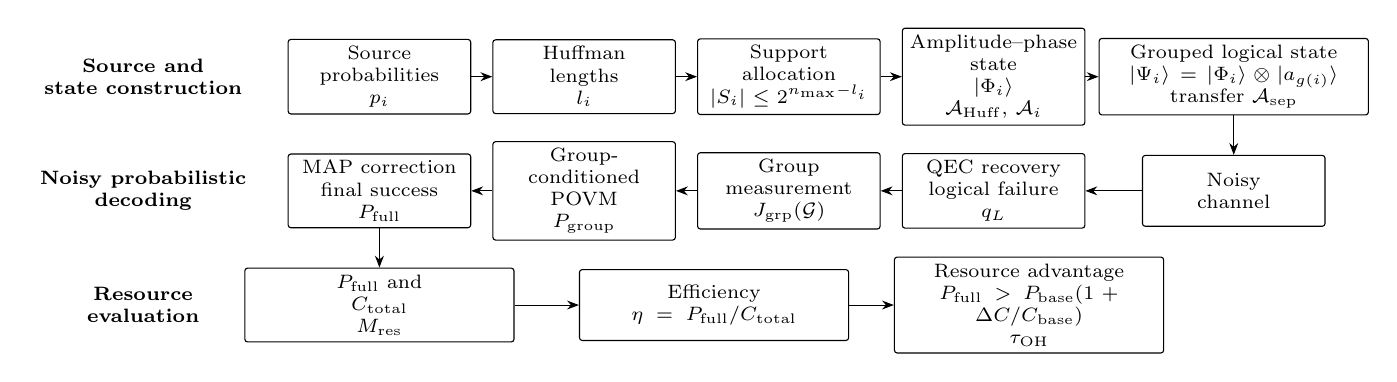
\begin{tikzpicture}[
    box/.style={draw, rounded corners=1pt, align=center, inner sep=2.4pt, font=\scriptsize, minimum height=9mm, text width=2.15cm},
    widebox/.style={draw, rounded corners=1pt, align=center, inner sep=2.4pt, font=\scriptsize, minimum height=9mm, text width=3.25cm},
    label/.style={font=\scriptsize\bfseries, align=center, text width=2.70cm},
    arr/.style={-{Stealth[length=1.5mm]}, line width=0.35pt}
]
\node[label] (lab1) at (0,0) {Source and\\state construction};
\node[box] (p) at (3.00,0) {Source\\probabilities\\$p_i$};
\node[box] (l) at (5.60,0) {Huffman\\lengths\\$l_i$};
\node[box] (s) at (8.20,0) {Support\\allocation\\$|S_i|\leq2^{n_{\max}-l_i}$};
\node[box] (phi) at (10.80,0) {Amplitude--phase\\state\\$\ket{\Phi_i}$\\$\mathcal A_{\mathrm{Huff}},\,\mathcal A_i$};
\node[widebox] (psi) at (13.85,0) {Grouped logical state\\$\ket{\Psi_i}=\ket{\Phi_i}\otimes\ket{a_{g(i)}}$\\transfer $\mathcal A_{\mathrm{sep}}$};
\node[label] (lab2) at (0,-1.45) {Noisy probabilistic\\decoding};
\node[box] (map) at (3.00,-1.45) {MAP correction\\final success\\$P_{\mathrm{full}}$};
\node[box] (povm) at (5.60,-1.45) {Group-conditioned\\POVM\\$P_{\mathrm{group}}$};
\node[box] (meas) at (8.20,-1.45) {Group\\measurement\\$J_{\mathrm{grp}}(\mathcal G)$};
\node[box] (qec) at (10.80,-1.45) {QEC recovery\\logical failure\\$q_L$};
\node[box] (noise) at (13.85,-1.45) {Noisy\\channel};
\node[label] (lab3) at (0,-2.90) {Resource evaluation};
\node[widebox] (cost) at (3.00,-2.90) {$P_{\mathrm{full}}$ and\\$C_{\mathrm{total}}$\\$M_{\rm res}$};
\node[widebox] (eta) at (7.25,-2.90) {Efficiency\\$\eta=P_{\mathrm{full}}/C_{\mathrm{total}}$};
\node[widebox] (adv) at (11.25,-2.90) {Resource advantage\\$P_{\mathrm{full}}>P_{\mathrm{base}}(1+\Delta C/C_{\mathrm{base}})$\\$\tau_{\mathrm{OH}}$};
\draw[arr] (p) -- (l); \draw[arr] (l) -- (s); \draw[arr] (s) -- (phi); \draw[arr] (phi) -- (psi);
\draw[arr] (psi.south) -- (noise.north); \draw[arr] (noise) -- (qec); \draw[arr] (qec) -- (meas); \draw[arr] (meas) -- (povm); \draw[arr] (povm) -- (map);
\draw[arr] (map.south) -- (cost.north); \draw[arr] (cost) -- (eta); \draw[arr] (eta) -- (adv);
\end{tikzpicture}}
\caption{\label{fig:pipeline}Pipeline of the proposed finite-resource probabilistic source-decoding framework. Huffman lengths define support budgets in a common Hilbert space. The allocated supports define amplitude--phase states $\ket{\Phi_i}$ and the ambiguity diagnostics \(\mathcal A_{\mathrm{Huff}}\) and \(\mathcal A_i\); group labels form $\ket{\Psi_i}=\ket{\Phi_i}\otimes\ket{a_{g(i)}}$ and transfer inter-group ambiguity into orthogonal label information measured by \(\mathcal A_{\mathrm{sep}}\). The grouping criterion \(J_{\mathrm{grp}}\) summarizes the resource-aware design trade-off. After noisy transmission, QEC recovery, group-conditioned POVM decoding, and MAP post-processing, the final success probability and modeled resource cost determine \(\eta\), the resource margin \(M_{\rm res}\), and the overhead tolerance \(\tau_{\mathrm{OH}}\).}
\end{figure*}

\section{Huffman-Induced Support Geometry}
\label{sec:support_geometry}

Let $\mathcal S=\{s_i\}_{i=1}^M$ be a discrete source with probabilities $p_i>0$ and $\sum_i p_i=1$. A classical Huffman tree assigns positive integer lengths $l_i$ satisfying Eq.~\eqref{eq:kraft_intro}. Here $l_i$ is a source-dependent support-budget parameter in a common ambient Hilbert space, with the integer $n_{\max}\geq\max_i l_i$ chosen so that every support budget is nonzero,
\begin{equation}
    \mathcal H_{\max}=(\mathbb C^2)^{\otimes n_{\max}}.
\end{equation}
For each symbol, choose a computational-basis support $S_i\subseteq\{0,1\}^{n_{\max}}$ obeying
\begin{equation}
    |S_i|\le 2^{n_{\max}-l_i}.
    \label{eq:huffman_support_size}
\end{equation}
Equivalently,
\begin{equation}
    \log_2|S_i|\le n_{\max}-l_i,
\end{equation}
with the saturated convention $l_i=n_{\max}-\log_2|S_i|$ when the budget is filled. Thus $l_i$ is a codimension-like support restriction in the chosen computational basis.
Kraft compatibility follows immediately:
\begin{equation}
    \sum_i |S_i|\le \sum_i2^{n_{\max}-l_i}=2^{n_{\max}}\sum_i2^{-l_i}\le 2^{n_{\max}}.
    \label{eq:support_kraft_compatibility}
\end{equation}
Thus the classical source distribution induces a feasible support geometry in a single Hilbert space. A local symbol-dependent representation with $n_i=f_n(l_i)$ may be useful for implementation, but all states compared by the decoder are understood to be embedded into $\mathcal H_{\max}$ by zero padding or an isometry. Detailed local representations and amplitude--phase gradients are collected in Appendix~\ref{app:gradients}.

\begin{proposition}[Support allocation]\label{prop:support-allocation}\hfill\par
For any Kraft-compatible positive integer length assignment and any integer \(n_{\max}\geq\max_i l_i\), disjoint supports of cardinality \(2^{n_{\max}-l_i}\) exist inside \(\mathcal H_{\max}\). Hence any smaller positive integer support budgets obeying Eq.~\eqref{eq:huffman_support_size} are also feasible.
\end{proposition}
\textit{Proof.} Set \(b_i=2^{n_{\max}-l_i}\), which is a positive integer under the stated assumptions. Kraft's inequality gives \(\sum_i b_i\leq 2^{n_{\max}}\), so the ambient computational basis can be partitioned into disjoint subsets of cardinalities \(b_i\), with any unused basis labels left unassigned. Choosing smaller positive integer cardinalities preserves feasibility. Overlapping subsets relax the requirement on distinct basis labels, while the disjoint construction already establishes Kraft feasibility. \(\square\)

The proposition establishes feasibility of the classical Kraft constraint in a common Hilbert space. After this support geometry is fixed, the amplitudes, phases, grouping, and POVM certificates determine whether the support saving survives discrimination and resource normalization.

Support overlap is compatible with Kraft allocation and provides an additional design degree of freedom. It determines where nonzero inner products are possible, while amplitudes and phases determine their actual values. We quantify support overlap by
\begin{equation}
    R_{\rm sup}
    =
    \frac{\sum_{i<j}|S_i\cap S_j|}
    {\sum_{i<j}\min(|S_i|,|S_j|)},
    \label{eq:support_overlap_ratio}
\end{equation}
with \(R_{\rm sup}=0\) when the denominator is zero. Three regimes are useful. In a disjoint-support regime, payload states are orthogonal and discrimination becomes easy, but the example no longer stresses probabilistic nonorthogonal decoding. In the overlap-controlled regime targeted here, support overlap permits finite ambiguity while group labels can transfer inter-group ambiguity into orthogonal label information. In an overlap-heavy regime, \(\mathcal A_{\rm Huff}\) can become too large and any support-budget saving may be lost after resource normalization.

\begin{definition}[Huffman-budget ensemble]\label{def:huffman-ensemble}
Fix $p$, $l$, $\mathcal H_{\max}$, and supports satisfying Eq.~\eqref{eq:huffman_support_size}. Define
\begin{equation}
    \begin{split}
    \mathcal E_{\rm Huff}=
    \{\,\{\ket{\Phi_i}\}_{i=1}^M:\;&
    {\rm supp}(\ket{\Phi_i})\subseteq S_i,\\
    &\braket{\Phi_i|\Phi_i}=1\,\}.
    \end{split}
\end{equation}
The ambiguity-minimizing payload design is
\begin{equation}
    \mathcal A_{\rm Huff}^{\star}
    =
    \min_{\{\ket{\Phi_i}\}\in\mathcal E_{\rm Huff}(p,l,S)}
    \sum_{i<j}p_ip_j|\braket{\Phi_i|\Phi_j}|^2 .
    \label{eq:AHuff_star}
\end{equation}
\end{definition}

The optimization in Eq.~\eqref{eq:AHuff_star} is generally nonconvex. The numerical ``optimized'' payload uses a deterministic local phase-search heuristic for this objective. Random-phase and deterministic-phase payloads are baselines for the same feasible class. The two-dimensional angle-defined four-symbol states used later provide a transparent sanity check; the main numerical studies use the support-constrained payload construction.

\paragraph*{Construction.}
The source-to-ensemble map used in the rest of the paper is as follows. Given a source distribution $\{p_i\}_{i=1}^M$, construct a classical Huffman tree and record the associated lengths $l_i$. Choose an ambient logical Hilbert space $\mathcal H_{\max}$ large enough to contain supports satisfying Eq.~\eqref{eq:huffman_support_size}. Assign computational-basis subsets $S_i\subseteq\{0,1\}^{n_{\max}}$ with total size compatible with Eq.~\eqref{eq:support_kraft_compatibility}. Inside each support, choose amplitudes and phases to form $\ket{\Phi_i}$, and compute the overlap matrix
\begin{equation}
    \Gamma_{ij}=\braket{\Phi_i|\Phi_j}.
\end{equation}
The matrix $\Gamma$ is the object passed to the grouping stage: groups are chosen so that highly ambiguous pairs are preferentially separated by the group ancilla, while the remaining intra-group states are decoded by conditional POVMs. Thus the Huffman tree affects decoding through support geometry and overlap structure.

This construction also clarifies the role of the ambient dimension. A larger $n_{\max}$ creates more possible basis supports and therefore more freedom to separate high-priority states. The modeled logical support cost remains tied to $\bar L$, and the physical redundancy cost enters separately through $C_{\mathrm{QEC}}$. Related source-coding work shows that ensemble structure and nondisturbing operations can be central to quantum compressibility~\cite{koashi2001compressibility,koashi2002operations}; here those ideas motivate a finite support-allocation design.

Within $S_i$ we use an amplitude--phase state
\begin{equation}
    \begin{aligned}
    \ket{\Phi_i}&=\sum_{x\in S_i} a_{i,x}e^{i\theta_{i,x}}\ket{x},\\
    a_{i,x}&\geq0,\qquad \theta_{i,x}\in\mathbb R,\qquad
    \sum_{x\in S_i}a_{i,x}^2=1 .
    \end{aligned}
    \label{eq:phi_state_main}
\end{equation}
The pairwise overlaps
\begin{equation}
    \braket{\Phi_i|\Phi_j}=\sum_{x\in S_i\cap S_j}a_{i,x}a_{j,x}e^{i(\theta_{j,x}-\theta_{i,x})}
    \label{eq:pairwise_overlap_main}
\end{equation}
control distinguishability. Numerically, the amplitude--phase design minimizes a weighted overlap surrogate such as
\begin{equation}
    \mathcal O=\sum_{i<j}p_ip_j|\braket{\Phi_i|\Phi_j}|^2,
    \label{eq:overlap_objective_main}
\end{equation}
which serves as a design proxy for the later optimal POVM stage. The formal contribution is the support geometry and its effect on the discrimination problem.
We will refer to the same source-weighted quantity as the Huffman-induced ambiguity budget,
\begin{equation}
    \mathcal A_{\mathrm{Huff}}
    =
    \sum_{i<j}p_ip_j|\braket{\Phi_i|\Phi_j}|^2,
    \label{eq:huffman_ambiguity_budget}
\end{equation}
with symbol-level contribution
\begin{equation}
    \mathcal A_i
    =
    p_i\sum_{j\neq i}p_j|\braket{\Phi_i|\Phi_j}|^2 .
    \label{eq:symbol_ambiguity_contribution}
\end{equation}
\(\mathcal A_{\mathrm{Huff}}\) measures the state-overlap ambiguity of the support-constrained ensemble, including its amplitude and phase choices, while large \(\mathcal A_i\) identifies source symbols that dominate the ambiguity budget. These diagnostic quantities guide support refinement and group design, and the optimal POVM/SDP decoder determines success probability.

The overlap objective in Eq.~\eqref{eq:overlap_objective_main} is useful because minimum-error discrimination is sensitive to pairwise and collective state geometry. Lowering the weighted overlaps of high-priority symbols can increase the value of the later POVM SDP, especially after grouping removes inter-group pairs from the conditional tasks. The optimization forms a state-design layer between source statistics and the optimal quantum decoder.

The formal analysis admits any feasible choice of amplitudes, phases, and supports. A deterministic implementation may use a fixed design heuristic, while an offline numerical study may optimize Eq.~\eqref{eq:overlap_objective_main}. In both cases the decoder sees the resulting finite ensemble \(\{p_i,\ket{\Phi_i}\}\), so the SDP-certified advantage theorem in Sec.~\ref{sec:resource_advantage} is independent of the particular amplitude--phase optimizer.

There are therefore three distinct design degrees of freedom. The Huffman tree fixes the support budgets, while the support assignment fixes which computational-basis components can contribute to overlap. The amplitude--phase choice then controls interference inside the shared portions of those supports. The first step is inherited directly from the classical source code; the latter two are quantum state-design choices evaluated by the downstream discrimination and resource tests.

\paragraph*{Numerical state-generation protocol.}
The numerical state-generation protocol is as follows. (i) Given \(p_i\), compute Huffman lengths \(l_i\), \(n_{\rm fix}=\lceil\log_2M\rceil\), and a common \(n_{\max}\). (ii) Allocate cyclic computational-basis supports satisfying \(|S_i|\le 2^{n_{\max}-l_i}\), allowing overlaps among payload states in the common Hilbert space. (iii) Generate payload states on these supports in three modes: an optimized phase search minimizing \(\mathcal A_{\rm Huff}\), a random-phase ensemble averaged over fixed seeds, and a deterministic-phase baseline. (iv) Form random, probability-aware, and overlap-aware group partitions and evaluate \(\mathcal A_{\rm in}\), \(\mathcal A_{\rm sep}\), \(P_{\rm group}\), \(P_{\rm full}\), \(\eta\), and \(M_{\rm res}\). (v) For certificate runs, solve numerically tractable small-instance SDPs and record \(\underline P_{\rm group}\), \(\overline P_{\rm fix}\), feasibility residuals, and \(M_{\rm cert}\).

\section{Group-Ancilla Conditional Discrimination}
\label{sec:group_discrimination}

Partition the source alphabet into groups $\mathcal G_g$ with group map $g(i)$. Attach an orthonormal ancilla label $\{\ket{a_g}\}_{g=1}^G$ and define
\begin{equation}
    \ket{\Psi_i}=\ket{\Phi_i}\otimes\ket{a_{g(i)}}.
    \label{eq:psi_group_state_main}
\end{equation}
Then
\begin{equation}
    \braket{\Psi_i|\Psi_j}=\braket{\Phi_i|\Phi_j}\delta_{g(i),g(j)},
    \label{eq:group_orthogonality_main}
\end{equation}
so inter-group alternatives become orthogonal while intra-group nonorthogonality remains. The ancilla changes the ensemble presented to each conditional decoder.

The same effect can be summarized as an ambiguity-budget transfer. Define
\begin{align}
    \mathcal A_{\mathrm{global}}
    &=
    \sum_{i<j}p_ip_j|\braket{\Phi_i|\Phi_j}|^2,\nonumber\\
    \mathcal A_{\mathrm{in}}
    &=
    \sum_g\sum_{\substack{i<j\\ i,j\in\mathcal G_g}}
    p_ip_j|\braket{\Phi_i|\Phi_j}|^2,\nonumber\\
    \mathcal A_{\mathrm{sep}}
    &=
    \mathcal A_{\mathrm{global}}-\mathcal A_{\mathrm{in}} .
    \label{eq:ambiguity_budget_transfer}
\end{align}
Here \(\mathcal A_{\mathrm{global}}\) is the overlap-weighted ambiguity carried by the original nonorthogonal ensemble, \(\mathcal A_{\mathrm{in}}\) is the part remaining inside conditional POVM tasks, and \(\mathcal A_{\mathrm{sep}}\) is the portion removed by converting inter-group alternatives into orthogonal label information. Like the overlap-ratio quantities in Appendix~\ref{app:supplementary_diagnostics}, \(\mathcal A_{\mathrm{sep}}\) is a group-design diagnostic; success probability is determined by the conditional decoder.

Operationally, the group measurement is performed before the conditional payload measurement. A conditional POVM is the family of payload measurements selected after the group outcome is known. If the outcome is $g$, all symbols outside $\mathcal G_g$ are eliminated without ambiguity, and group-conditioned discrimination is the resulting smaller minimum-error task with renormalized priors $p_i/p_g$. This is the sense in which grouping converts one global nonorthogonal ensemble into a family of conditional ensembles.

After measuring the group label, group $g$ occurs with probability $p_g=\sum_{i\in\mathcal G_g}p_i$. The optimal conditional success is the minimum-error discrimination SDP
\begin{align}
    P_{\mathrm{opt}}^{(g)}
    =
    \max_{\{E_i^{(g)}\}}
    &\sum_{i\in\mathcal G_g}
    \frac{p_i}{p_g}
    \operatorname{Tr}(E_i^{(g)}\rho_i^{(g)})
    \label{eq:group_sdp_main}\\
    \text{subject to}\quad
    &E_i^{(g)}\succeq0,\qquad
    \sum_{i\in\mathcal G_g}E_i^{(g)}=I_g .
    \nonumber
\end{align}
The grouped success is
\begin{equation}
    P_{\mathrm{group}}=\sum_g p_gP_{\mathrm{opt}}^{(g)}.
    \label{eq:p_group_main}
\end{equation}
The Helstrom two-state check is given in Appendix~\ref{app:sdp_validation}, while the primal-dual SDP details and KKT conditions are given in Appendix~\ref{app:qec_sdp_details}.

\begin{proposition}[Group-label guessing floor]\label{prop:group-guess-floor}
With access to the orthogonal group label,
\begin{equation}
    P_{\mathrm{group}}\ge \sum_g \max_{i\in\mathcal G_g}p_i .
    \label{eq:group_guess_floor}
\end{equation}
\end{proposition}
\textit{Proof.} After measuring the group label, the receiver knows that the symbol lies in $\mathcal G_g$. A feasible conditional strategy is to ignore the payload state and always guess the most likely symbol in that group. Its conditional success is $\max_{i\in\mathcal G_g}p_i/p_g$. Averaging over $g$ gives $\sum_g p_g\max_{i\in\mathcal G_g}(p_i/p_g)=\sum_g\max_{i\in\mathcal G_g}p_i$. The optimal POVM decoder within each group achieves at least this value. \(\square\)

For \(G=1\), this reduces to the ordinary prior-guessing floor \(\max_i p_i\). For \(G=M\), the orthogonal label provides complete side information and the bound equals one, with its label cost charged through \(C_A\).

\begin{theorem}[Ideal group-label non-degradation]\label{thm:group-nondegradation}
Let \(P_{\mathrm{base}}\) here denote the optimal minimum-error success for the same priors and payload ensemble when the receiver does not use the group label. If the receiver has access to the orthogonal group label and may implement the optimal conditional POVM inside each group, then \(P_{\mathrm{group}}\geq P_{\mathrm{base}}\).
\end{theorem}
\textit{Proof.} Let \(\{F_i\}_{i=1}^M\) be an optimal payload POVM for the unlabeled ensemble. After learning \(g\), the receiver may apply this same POVM and retain every outcome in \(\mathcal G_g\), while remapping outcomes outside \(\mathcal G_g\) to an arbitrary symbol in that group. This is a feasible conditional decision rule and preserves every success event of the original POVM, so its average success is at least \(P_{\mathrm{base}}\). The optimal conditional POVM achieves at least the same success. \(\square\)

This theorem concerns raw discrimination success for the same payload ensemble; the resource-normalized comparison additionally includes the group-label cost \(C_A\).

The ancilla cost used later is
\begin{equation}
    C_A=\lceil\log_2G\rceil .
    \label{eq:ancilla_cost}
\end{equation}
Increasing $G$ may reduce within-group overlap and lower the SDP complexity of each conditional task, but it also increases $C_A$ and may leave too few symbols per group to justify the extra label. The resource analysis therefore treats grouping as a tunable design choice.

In the numerical examples, groups are chosen by simple source-aware or overlap-aware heuristics. Their effect combines the exact removal of inter-group overlaps in Eq.~\eqref{eq:group_orthogonality_main} with the remaining intra-group discrimination difficulty. A poor partition can spend ancilla bits without reducing the hard overlaps, whereas a favorable partition concentrates the ambiguous pairs into smaller tasks where the conditional POVM can exploit the posterior priors.

The grouped decoder is therefore analyzed through conditional SDPs. The group measurement changes the feasible measurement strategy: once $g$ is known, the POVM only separates states inside $\mathcal G_g$. Pairwise overlap diagnostics guide design and visualization, while the conditional minimum-error problem determines success probability. The SDP-certified theorem uses this distinction by comparing a grouped primal certificate with a fixed-length dual certificate.

\paragraph*{Resource-aware group design.}
The grouping heuristics used in the diagnostics can be summarized by a compact design objective. For a partition \(\mathcal G=\{\mathcal G_g\}_{g=1}^G\), define
\begin{align}
    J_{\mathrm{grp}}(\mathcal G)
    &=
    \alpha\,\mathcal A_{\mathrm{in}}(\mathcal G)
    +
    \beta\,\epsilon_{\mathrm{in}}(\mathcal G)
    +
    \gamma\,C_A(\mathcal G), \nonumber\\
    \epsilon_{\mathrm{in}}(\mathcal G)
    &=
    \max_g\max_{\substack{i\ne j\\ i,j\in\mathcal G_g}}
    |\braket{\Phi_i|\Phi_j}|^2,\nonumber\\
    C_A(\mathcal G)
    &=
    \lceil\log_2G\rceil .
    \label{eq:resource_aware_group_objective}
\end{align}
Here \(\mathcal A_{\mathrm{in}}(\mathcal G)\) penalizes prior-weighted intra-group ambiguity, \(\epsilon_{\mathrm{in}}(\mathcal G)\) penalizes the worst within-group overlap, and \(C_A(\mathcal G)\) penalizes group-label overhead; \(\alpha,\beta,\gamma\) are design weights. Equation~\eqref{eq:resource_aware_group_objective} provides a design criterion, and the numerical diagnostics use random, probability-aware, and overlap-aware heuristics for the broader resource-aware group design problem.

\section{QEC-Assisted Probabilistic Decoding}
\label{sec:qec_prob_decoding}

The QEC component provides an effective reliability abstraction that includes logical-failure suppression and redundancy cost under an architecture-independent model~\cite{nielsen2010quantum,terhal2015quantum}.

Noise is modeled at the logical ensemble level. A QEC layer is represented by an isometric encoding $V_{\mathrm{QEC}}$, a noisy channel, and a recovery map. Ideal encoding preserves logical inner products, while recovery suppresses additional channel-induced failures. Syndrome projectors, correctable error sets, and stabilizer-code bounds are given in Appendix~\ref{app:qec_sdp_details}.

For group $g$, let $q_L^{(g)}$ be the effective logical failure probability after recovery and let $P_{\mathrm{fallback}}^{(g)}$ be the success probability of the declared fallback decision rule after an uncorrectable event. The parameter $q_L^{(g)}$ is a modular interface to a recovery model: a hardware-specific logical channel may replace it without changing the support or discrimination layers. The QEC-assisted lower bound used throughout the paper is
\begin{equation}
    P_{\mathrm{full}}
    \ge
    \sum_g p_g\left[(1-q_L^{(g)})P_{\mathrm{opt}}^{(g)}+q_L^{(g)}P_{\mathrm{fallback}}^{(g)}\right].
    \label{eq:full_bound_main}
\end{equation}
When the effective failure probability and fallback success are assumed source- and group-independent, $q_L^{(g)}=q_L$ and $P_{\mathrm{fallback}}^{(g)}=P_{\mathrm{fallback}}$, this reduces to
\begin{equation}
    P_{\mathrm{full}}\ge (1-q_L)P_{\mathrm{group}}+q_LP_{\mathrm{fallback}}.
    \label{eq:full_bound_simple_main}
\end{equation}
A prior-only MAP fallback in group \(g\) attains
\begin{equation}
    P_{\mathrm{fallback}}^{(g)}
    =
    \max_{i\in\mathcal G_g}\frac{p_i}{p_g},
    \label{eq:map_aware_fallback_floor}
\end{equation}
and any optimized fallback with additional information can do at least as well, whereas the illustrative binary-group diagnostics retain the conservative random fallback \(P_{\mathrm{fallback}}=1/2\).
The resource analysis uses the QEC layer through this effective logical-failure model.

For a compact stabilizer-code reliability proxy, let an $[[n,k,d]]$ code correct up to
\begin{equation}
    t=\left\lfloor\frac{d-1}{2}\right\rfloor
    \label{eq:t_correct_main}
\end{equation}
errors under an independent physical-error model with error probability $p$. Specifically, the binomial proxy assumes independent occurrences of a specified error family and correction of every error of weight at most $t$ in that family. Under those assumptions, the correctable-event probability is bounded by
\begin{equation}
    P_{\mathrm{corr}}
    \ge
    \sum_{w=0}^{t}
    \binom{n}{w}p^w(1-p)^{n-w},
    \label{eq:pcorr_proxy_main}
\end{equation}
With the logical failure probability defined by
\begin{equation}
    q_L=1-P_{\mathrm{corr}},
    \label{eq:ql_definition_main}
\end{equation}
it follows that
\begin{equation}
    q_L
    \le
    1-
    \sum_{w=0}^{t}
    \binom{n}{w}p^w(1-p)^{n-w}.
    \label{eq:ql_proxy_main}
\end{equation}
This binomial expression serves as a finite-resource stabilizer-code reliability proxy. Hardware-calibrated fault-tolerant analyses require architecture-specific overhead and threshold modeling~\cite{fowler2012surface,terhal2015quantum,campbell2017roads}. Syndrome-level modeling and the associated correctable-error notation are given in Appendix~\ref{app:qec_sdp_details}~\cite{shor1995scheme,steane1996error,calderbank1996good,gottesman1997stabilizer,lidar2013quantum}.

Equation~\eqref{eq:full_bound_main} has a simple interpretation. With probability $1-q_L^{(g)}$, the recovered state is treated as being in the intended logical ensemble for group $g$, and the conditional POVM succeeds with probability $P_{\mathrm{opt}}^{(g)}$. With probability $q_L^{(g)}$, the decoder falls back to a conservative decision rule. This abstraction is intentionally coarse: it captures the reliability benefit of error correction without asserting a hardware-calibrated recovery circuit.

Given the classical observation tuple $y=(g,z,r)$, comprising the group-label outcome $g$, conditional-POVM outcome $z$, and syndrome/recovery flag $r$, the MAP post-processing rule is
\begin{equation}
    \hat i_{\mathrm{MAP}}(y)=\arg\max_i p_i P(y|i).
    \label{eq:map_rule_main}
\end{equation}
For fixed local observations and priors, this rule minimizes block-local decision error. Indeed, for any deterministic post-processing rule \(D\), the conditional probability of a correct decision at observation \(y\) is \(P(D(y)|y)\). Since this quantity is maximized pointwise by choosing the posterior maximizer, the MAP rule is optimal among block-local deterministic decision rules. Its contribution comes from additional classical information in $y$, such as the group or recovery outcome, and forms the deterministic posterior step following probabilistic quantum decoding.

In the numerical diagnostics, $P_{\mathrm{fallback}}$ is chosen consistently with the same posterior information available after failure. MAP correction affects the final deterministic decision rule, while the support allocation, group orthogonality, and SDP certificates remain fixed. Thus support geometry and grouping define the ensemble; POVM/SDP gives optimal probabilistic decoding; QEC changes the effective reliability; and MAP chooses the final symbol from the posterior.

Two forms of \(q_L\) are used in the paper. The main figures use compact effective logical-failure curves so that the resource trade-off can be inspected directly. The appendices record the corresponding repetition-style toy model and standard stabilizer-code upper bounds. These models supply controlled reliability parameters for Eq.~\eqref{eq:full_bound_main}. A hardware-specific recovery model can replace \(q_L\) while preserving the support-allocation and group-conditioned decoding layers.

\section{Resource-Aware Advantage Conditions}
\label{sec:resource_advantage}

The resource model is an abstract scalarized accounting convention that assigns commensurate unit weights to the modeled resources. This finite-resource accounting follows a one-shot resource comparison~\cite{tomamichel2013hierarchy,tomamichel2016finite}. Since Huffman lengths are support-budget parameters, the cost
\begin{equation}
    C_{\mathrm{total}}=\bar L+C_A+C_{\mathrm{QEC}}
    \label{eq:total_resource}
\end{equation}
uses $\bar L$ as the Huffman-induced average logical support-budget cost, $C_A$ as the group-label cost, and $C_{\mathrm{QEC}}$ as modeled physical redundancy. It is a comparison proxy under this declared convention. The efficiency is
\begin{equation}
    \eta=\frac{P_{\mathrm{success}}}{C_{\mathrm{total}}}.
    \label{eq:eta_main}
\end{equation}
and is consequently convention dependent.

The distinction between \(P_{\mathrm{group}}\) and \(P_{\mathrm{full}}\) is important: \(P_{\mathrm{group}}\) is a discrimination quantity for the recovered logical ensemble, while \(P_{\mathrm{full}}\) includes the reliability fallback model. Likewise, \(C_{\mathrm{QEC}}\) and \(\bar L\) separately represent physical redundancy and logical support budgeting. This separation is consistent with fault-tolerant architectures where improved logical reliability typically comes with substantial physical-resource overhead~\cite{fowler2012surface,campbell2017roads}.

The final resource test follows directly from comparing efficiencies. Let $C_{\mathrm{base}}>0$ and $C_{\mathrm{base}}+\Delta C>0$, and define
\begin{equation}
    \eta_{\mathrm{base}}=\frac{P_{\mathrm{base}}}{C_{\mathrm{base}}},
    \qquad
    \eta_{\mathrm{full}}=\frac{P_{\mathrm{full}}}{C_{\mathrm{base}}+\Delta C}.
    \label{eq:eta_base_full_derivation}
\end{equation}
Under the metric \(\eta=P_{\mathrm{success}}/C_{\mathrm{total}}\), the full scheme is resource-superior to the baseline if and only if
\(\eta_{\mathrm{full}}>\eta_{\mathrm{base}}\). Rearranging this necessary and sufficient condition gives
\begin{equation}
    P_{\mathrm{full}}>P_{\mathrm{base}}\left(1+\frac{\Delta C}{C_{\mathrm{base}}}\right),
    \label{eq:resource_advantage_condition}
\end{equation}
or equivalently, with \(\Delta P=P_{\mathrm{full}}-P_{\mathrm{base}}\),
\begin{equation}
    \Delta P>\frac{P_{\mathrm{base}}\Delta C}{C_{\mathrm{base}}}.
    \label{eq:delta_p_resource_condition}
\end{equation}
Thus the success increase must exceed the baseline success multiplied by the fractional resource overhead.
Equivalently, the resource margin
\begin{equation}
    M_{\rm res}
    =
    P_{\mathrm{full}}
    -
    P_{\mathrm{base}}
    \left(1+\frac{\Delta C}{C_{\mathrm{base}}}\right)
    \label{eq:resource_margin_main}
\end{equation}
is positive exactly when the full scheme is resource-superior under this accounting convention. A nonpositive margin means that reliability gain alone is insufficient to certify advantage in the metric of Eq.~\eqref{eq:eta_main}. In the numerical phase diagrams, \(P_{\mathrm{base}}\) is instantiated by the numerically solved SDP or representative baseline \(P_{\mathrm{base,opt}}\), so the plotted margin is the same diagnostic with that baseline substituted.
For \(P_{\mathrm{base}}>0\), solving Eq.~\eqref{eq:resource_advantage_condition} for the allowed relative overhead gives
\begin{equation}
    \frac{\Delta C}{C_{\mathrm{base}}}
    <
    \tau_{\mathrm{OH}},
    \qquad
    \tau_{\mathrm{OH}}
    =
    \frac{P_{\mathrm{full}}}{P_{\mathrm{base}}}-1 .
    \label{eq:overhead_tolerance}
\end{equation}
The quantity \(\tau_{\mathrm{OH}}\) is the overhead tolerance of the full decoder under the stated finite-resource accounting convention. Relative overhead below this model-specific diagnostic threshold satisfies the corresponding resource test.

A source-coding baseline is obtained from $n_{\mathrm{fix}}=\lceil\log_2M\rceil$ and
\begin{equation}
    G_{\mathrm{comp}}=n_{\mathrm{fix}}-\bar L.
\end{equation}
Here $n_{\mathrm{fix}}$ is the fixed-length logical cost of assigning every symbol the same binary label length, while $\bar L$ is the average support-budget cost inherited from the Huffman allocation. Thus $G_{\mathrm{comp}}$ measures average logical support saving. The standard Huffman inequality $H(p)\le \bar L < H(p)+1$ implies that nonuniform sources can give positive average support saving, especially when $H(p)$ is well below $\log_2M$. Resource advantage additionally requires sufficient state distinguishability to preserve the success gain.

For example, for \(P_{\mathrm{fix}}>0\), comparing a Huffman-induced grouped decoder with a fixed-length grouped decoder under the same ancilla and QEC accounting gives the sufficient condition
\begin{equation}
    \frac{P_{\mathrm{full}}}{P_{\mathrm{fix}}}
    >
    \frac{\bar L+C_A+C_{\mathrm{QEC}}}
    {n_{\mathrm{fix}}+C_A+C_{\mathrm{QEC}}}.
    \label{eq:huff_fixed_cost_comparison}
\end{equation}
This inequality makes explicit the trade-off: Huffman support budgeting helps through the denominator, while grouping and QEC must protect the numerator.

The baseline $P_{\mathrm{fix}}$ can be instantiated in several ways. In an analytic comparison it may be a fixed-length ensemble satisfying a bounded-overlap model. In a numerical comparison it may be the numerically solved SDP value $P_{\mathrm{base,opt}}$ for a fixed representation, or a controlled approximation such as a pretty-good measurement for larger randomized ensembles. What matters for Eq.~\eqref{eq:huff_fixed_cost_comparison} is that the success probability and the cost are evaluated under the same accounting convention.

The minimal logical accounting convention used in most formulas is
\begin{equation}
    C_{\rm total}=\bar L+C_A+C_{\rm QEC}.
\end{equation}
To expose platform sensitivity, the numerical diagnostics also scan the weighted model
\begin{equation}
    \begin{split}
    C_{\rm total}^{(w)}
    ={}& w_L\bar L+w_AC_A+w_QC_{\rm QEC}\\
    &+w_DD+w_MN_{\rm meas}+w_GN_{\rm gate}.
    \end{split}
    \label{eq:weighted_resource_model}
\end{equation}
The minimal convention is the special case \(w_L=w_A=w_Q=1\) and \(w_D=w_M=w_G=0\). The corresponding diagnostics use
\begin{equation}
    \eta^{(w)}=\frac{P_{\rm full}}{C_{\rm total}^{(w)}},
    \qquad
    M_{\rm res}^{(w)}
    =
    P_{\rm full}
    -
    P_{\rm base}\frac{C_{\rm total}^{(w)}}{C_{\rm base}^{(w)}}.
\end{equation}
The weights \(w_L,w_A,w_Q,w_D,w_M,w_G\) are nonnegative, and the weighted comparisons are made only when \(C_{\rm total}^{(w)}>0\) and \(C_{\rm base}^{(w)}>0\). Their ratios declare how unlike resources are scalarized. Conclusions that change across plausible weights are convention sensitive. Weighted robustness therefore provides a sensitivity diagnostic for the declared accounting convention.

\begin{proposition}[No-free-lunch]\label{prop:no-free-lunch}\hfill\par
No unconditional resource-normalized advantage can hold for all source distributions and all admissible overhead models with positive cost denominators.
\end{proposition}
\textit{Proof.} For a uniform source on a power-of-two alphabet, the Huffman average support cost equals \(n_{\rm fix}\), so the support-budget saving \(G_{\rm comp}=n_{\rm fix}-\bar L\) vanishes; nearby sources make it arbitrarily small. If the group-label overhead, QEC overhead, depth cost, measurement cost, or gate cost is sufficiently large, then \(C_{\rm total}\) or \(C_{\rm total}^{(w)}\) can exceed the fixed baseline cost by enough to offset any raw success improvement. Therefore \(P_{\rm full}>P_{\rm base}\) can still coexist with \(\eta\le\eta_{\rm base}\), \(M_{\rm res}\le0\), or \(M_{\rm res}^{(w)}\le0\). Resource advantage therefore requires a finite-instance or parameter-regime certificate. \(\square\)

\subsection{Bounded-overlap analytic condition}

The bounded-overlap theorem provides a design rule for a comparison class in which pairwise ambiguity controls success in the conservative form written below. The optimal decoder remains the POVM/SDP decoder, while the overlap model exposes how source nonuniformity, group separation, and reduced within-group overlap can combine to yield a sufficient resource advantage.
The assumptions in Eqs.~\eqref{eq:fixed_overlap_bound_main} and \eqref{eq:group_overlap_bound_main} define this comparison class. A controlled fixed-overlap baseline is a fixed-length reference constructed to obey the stated overlap bound while other comparison choices are held fixed. Such baselines are useful in controlled-overlap numerical families or during preliminary design before a numerical SDP certificate is available. The SDP-certified theorem below uses direct primal and dual certificates.
Define
\begin{equation}
    \Lambda(p)=\sum_{i<j}p_ip_j=\frac{1-\sum_ip_i^2}{2},
\end{equation}
\begin{equation}
    \Lambda_{\mathrm{in}}(p,\mathcal G)=\sum_g\sum_{\substack{i<j\\ i,j\in\mathcal G_g}}p_ip_j\le \Lambda(p).
\end{equation}
Assume a fixed-length baseline comparison class with
\begin{equation}
    P_{\mathrm{fix}}\le 1-\epsilon_{\mathrm{fix}}\Lambda(p),
    \label{eq:fixed_overlap_bound_main}
\end{equation}
and a grouped Huffman-induced comparison class with
\begin{equation}
    P_{\mathrm{Huff+grp}}\ge 1-\epsilon_{\mathrm{in}}\Lambda_{\mathrm{in}}(p,\mathcal G).
    \label{eq:group_overlap_bound_main}
\end{equation}
Here \(0\leq\epsilon_{\mathrm{in}},\epsilon_{\mathrm{fix}}\leq1\), and $\epsilon_{\mathrm{in}}$ is an upper bound on the maximum within-group squared overlap, evaluated numerically as $\max_g\max_{i\ne j\in\mathcal G_g}|\braket{\Phi_i|\Phi_j}|^2$. Equations~\eqref{eq:fixed_overlap_bound_main} and \eqref{eq:group_overlap_bound_main} are explicit performance assumptions in addition to the maximum pairwise-overlap bound.

\begin{theorem}[Bounded-overlap advantage]\label{thm:bounded-overlap}
Let $n_{\mathrm{fix}}>0$ and $\bar L+C_A>0$. Suppose the fixed-length and grouped ensembles satisfy Eqs.~\eqref{eq:fixed_overlap_bound_main} and \eqref{eq:group_overlap_bound_main}, respectively, for the same prior $p$ and declared no-QEC cost convention. If
\begin{equation}
    \frac{1-\epsilon_{\mathrm{in}}\Lambda_{\mathrm{in}}(p,\mathcal G)}{\bar L+C_A}
    >
    \frac{1-\epsilon_{\mathrm{fix}}\Lambda(p)}{n_{\mathrm{fix}}}
    \label{eq:bounded_overlap_advantage_main}
\end{equation}
holds, then $\eta_{\mathrm{Huff+grp}}^{(0)}>\eta_{\mathrm{fix}}^{(0)}$.
\end{theorem}
\textit{Proof.} The assumed lower bound on $P_{\mathrm{Huff+grp}}$ gives a lower bound on $\eta_{\mathrm{Huff+grp}}^{(0)}=P_{\mathrm{Huff+grp}}/(\bar L+C_A)$, while the assumed upper bound on $P_{\mathrm{fix}}$ gives an upper bound on $\eta_{\mathrm{fix}}^{(0)}=P_{\mathrm{fix}}/n_{\mathrm{fix}}$. If Eq.~\eqref{eq:bounded_overlap_advantage_main} holds, the former lower bound exceeds the latter upper bound. \(\square\)

The low-overlap corollary is immediate: if $\bar L+C_A<n_{\mathrm{fix}}$ and $\epsilon_{\mathrm{in}}\le[(\bar L+C_A)/n_{\mathrm{fix}}]\epsilon_{\mathrm{fix}}$, then the strict inequality holds. Including QEC replaces the numerator by the lower bound in Eq.~\eqref{eq:full_bound_simple_main} and the denominator by $\bar L+C_A+C_{\mathrm{QEC}}$.

\subsection{SDP-certified resource advantage}

The SDP-certified theorem removes the bounded-overlap model. We use $P_{\mathrm{group}}$ for the ideal or computed grouped success and $\underline P_{\mathrm{group}}$ for any feasible lower certificate used in the SDP-certified comparison. Consider a fixed-length ensemble $\mathcal E_{\mathrm{fix}}=\{p_i,\rho_i^{\mathrm{fix}}\}_{i=1}^M$ with optimal success $P^\star_{\mathrm{fix}}$, and a Huffman-induced grouped ensemble with optimal grouped success $P_{\mathrm{group}}$. If feasible group POVMs provide a primal lower certificate $\underline P_{\mathrm{group}}\le P_{\mathrm{group}}$, and a dual feasible operator $Y$ satisfying
\begin{equation}
    Y\succeq p_i\rho_i^{\mathrm{fix}},\qquad i=1,\ldots,M,
\end{equation}
provides the upper certificate $\overline P_{\mathrm{fix}}=\operatorname{Tr}Y\ge P^\star_{\mathrm{fix}}$, then weak duality gives the following result.

\begin{theorem}[SDP-certified resource advantage]\label{thm:sdp-resource}
Fix the two ensembles and a common accounting convention with $n_{\mathrm{fix}}>0$ and $\bar L+C_A>0$. Suppose the grouped POVM is primal feasible with value $\underline P_{\mathrm{group}}$, and $Y$ is dual feasible for the fixed-length ensemble with $\overline P_{\mathrm{fix}}=\operatorname{Tr}Y\ge P^\star_{\mathrm{fix}}$. If
\begin{equation}
    \frac{\underline P_{\mathrm{group}}}{\bar L+C_A}>
    \frac{\overline P_{\mathrm{fix}}}{n_{\mathrm{fix}}},
    \label{eq:sdp_certificate_condition_main}
\end{equation}
then $\eta_{\mathrm{Huff+grp}}^{(0)}>\eta_{\mathrm{fix}}^{(0)}$.
\end{theorem}
\textit{Proof.} Primal feasibility gives $P_{\mathrm{group}}\ge\underline P_{\mathrm{group}}$, and fixed-length dual feasibility gives $P^\star_{\mathrm{fix}}\le\overline P_{\mathrm{fix}}$. Dividing by the corresponding positive costs and using Eq.~\eqref{eq:sdp_certificate_condition_main} yields the strict efficiency ordering. \(\square\)

For a concrete pair of ensembles, a fixed resource accounting convention, and feasible SDP certificates, a positive normalized certificate gap verifies strict resource advantage. The exact theorem yields numerical finite-instance certificates when the reported primal and dual objects pass the stated feasibility checks and residual tests. The positive cases reported in the Supplemental Material demonstrate that the sufficient condition is attained by explicit finite instances, while negative margins leave the ordering unresolved.
In the same certificate language, the normalized QEC-assisted certified margin may be written as
\begin{equation}
    M_{\rm cert}
    =
    \frac{\underline P_{\mathrm{full}}}{\bar L+C_A+C_{\mathrm{QEC}}}
    -
    \frac{\overline P_{\mathrm{fix}}}{n_{\mathrm{fix}}}.
    \label{eq:certified_margin_main}
\end{equation}
Positive \(M_{\rm cert}\) is the certificate form corresponding to the SDP-certified theorem: it compares a QEC-assisted grouped lower certificate with a fixed-length dual upper certificate under the same accounting convention and certifies the corresponding finite instance.

\begin{corollary}[QEC-assisted SDP certificate]\label{cor:qec-sdp}
Under the hypotheses of Theorem~\ref{thm:sdp-resource}, let $q_L\in[0,1]$, let $P_{\mathrm{fallback}}\in[0,1]$ be a valid fallback lower bound, let $C_{\mathrm{QEC}}\ge0$, and assume the source- and group-independent effective logical-failure model of Eq.~\eqref{eq:full_bound_simple_main}. Suppose the QEC-assisted effective success is certified by
\begin{equation}
    \underline P_{\mathrm{full}}
    =
    (1-q_L)\underline P_{\mathrm{group}}
    +
    q_LP_{\mathrm{fallback}} .
    \label{eq:qec_sdp_cert_main}
\end{equation}
If the value substituted for \(q_L\) is only a conservative upper bound \(\bar q_L\ge q_L^{\mathrm{true}}\), additionally require \(P_{\mathrm{fallback}}\le\underline P_{\mathrm{group}}\), so that replacing \(q_L^{\mathrm{true}}\) by \(\bar q_L\) preserves the lower-certificate direction. If \(q_L\) is treated directly as the specified effective-model parameter, no additional monotonicity assumption is required.
If
\begin{equation}
    \frac{\underline P_{\mathrm{full}}}
    {\bar L+C_A+C_{\mathrm{QEC}}}
    >
    \frac{\overline P_{\mathrm{fix}}}{n_{\mathrm{fix}}},
    \label{eq:qec_sdp_cert_condition_main}
\end{equation}
then the QEC-assisted Huffman-grouped decoder is certified to be more resource efficient than the fixed-length baseline under the same accounting convention.
\end{corollary}
\textit{Proof.} Equation~\eqref{eq:qec_sdp_cert_main} is a lower certificate for the full success under the effective logical-failure model, while $\overline P_{\mathrm{fix}}$ remains a dual upper certificate for the fixed-length baseline. Dividing by the respective costs gives the claimed strict ordering whenever Eq.~\eqref{eq:qec_sdp_cert_condition_main} holds. \(\square\)

The corollary certifies a sufficient condition for a specified ensemble, recovery model, and cost convention.

In practice the two resource theorems serve different purposes. The bounded-overlap condition is useful during design because it shows which levers matter before an SDP is solved: lower \(\bar L+C_A\), lower \(\epsilon_{\mathrm{in}}\), and higher baseline ambiguity all favor the grouped Huffman-induced construction. The SDP-certified condition is useful after a concrete ensemble has been built. A feasible grouped measurement gives \(\underline P_{\mathrm{group}}\), while a feasible dual variable for the fixed-length baseline gives \(\overline P_{\mathrm{fix}}\). If the normalized certificate gap is positive, the advantage claim is certified for that instance under the stated resource convention.

For a fixed source, support allocation and grouping determine the ensemble, after which the reliability model and normalized resource certificate are evaluated. A negative margin leaves the support construction intact and indicates that the chosen grouping, recovery model, and cost convention fail the sufficient resource-advantage test.

The fixed-length baseline may use an optimized POVM and, in the SDP-certified theorem, a dual upper certificate on its optimal success probability. The grouped construction supplies a feasible lower certificate, while the fixed-length baseline supplies an upper certificate. If the lower normalized value exceeds the upper normalized value, the strict advantage conclusion follows. If the inequality fails, the theorem leaves the ordering unresolved.

\section{Numerical Diagnostics}
\label{sec:numerical_results}

The numerical diagnostics follow the logical chain of the construction: support-budget saving, support-constrained payload generation, group ambiguity transfer, default resource-normalized benchmark, favorable-regime sweep, numerically solved certificate statistics, weighted sensitivity, and finally the auxiliary QEC/MAP layers. The benchmark tests representative behavior under a conservative cost convention; the sweep maps structured regions where the same resource inequalities become positive. SDP certificate rows provide finite-instance certificates, while larger scalable rows provide PGM diagnostics.

\subsection{Protocol and baselines}

All main-text diagnostics use the same accounting convention as Sec.~\ref{sec:resource_advantage}. The fixed-length reference has logical cost \(n_{\mathrm{fix}}\) and success denoted \(P_{\mathrm{base,opt}}\) when it is computed by a numerical SDP. The grouped Huffman-induced decoder has support cost \(\bar L+C_A\) before QEC and success \(P_{\mathrm{group}}\). With the effective reliability layer, the reported success is the lower-bound quantity \(P_{\mathrm{full}}\) from Eq.~\eqref{eq:full_bound_simple_main}, and the reported efficiency is
\begin{equation}
    \eta=\frac{P_{\mathrm{full}}}{\bar L+C_A+C_{\mathrm{QEC}}}.
\end{equation}
The notation \(P_{\mathrm{base,opt}}\) is reserved for the numerically solved SDP or representative baseline used in plots, whereas \(P^\star_{\mathrm{fix}}\) and \(\overline P_{\mathrm{fix}}\) are used in the SDP-certified theorem.
The phase diagrams visualize the resource margin
\begin{equation}
    M_{\rm res}
    =
    P_{\mathrm{full}}
    -
    P_{\mathrm{base,opt}}
    \left(1+\frac{\Delta C}{C_{\mathrm{base}}}\right),
    \label{eq:numerical_margin}
\end{equation}
which is Eq.~\eqref{eq:resource_margin_main} with \(P_{\mathrm{base}}\) replaced by the numerical baseline \(P_{\mathrm{base,opt}}\). Thus \(M_{\rm res}>0\) corresponds to the resource-advantage condition, while the boundary plots in Appendix~\ref{app:additional_phase} visualize the corresponding overhead tolerance \(\tau_{\mathrm{OH}}\).

The scalable multi-\(M\) benchmark uses the pretty-good measurement and is explicitly labeled as an approximate diagnostic in the CSV files. Numerically solved SDP certificates are reported for \(M=4\), while \(M=8\) and larger benchmark rows are marked as approximate. This distinction is important because the resource theorem is stated in terms of certificates, while the scalable simulations illustrate parameter regimes in which such certificates or lower bounds may be worth searching.

The fixed-length baseline is intentionally strong within each computational regime. It uses the same priors and the same payload ensemble where the goal is to isolate resource accounting, with fixed-length cost \(n_{\rm fix}\); for scalable rows this baseline is labeled \texttt{pgm\_fixed\_global}. Numerical SDP fixed-global baselines are used in the small certificate search. The benchmark CSV also includes \texttt{equal\_support} and \texttt{random\_support} rows as diagnostic support-allocation baselines under the same ambient dimension.

In a same-payload baseline, the payload ensemble is held fixed for the baseline comparison, while the accounting and group conditioning differ. This isolates the value and cost of the orthogonal group label without attributing the gain to a different set of payload states.

The effective QEC curves report the lower-bound proxy \((1-q_L)P_{\mathrm{group}}+q_LP_{\mathrm{fallback}}\) from Eq.~\eqref{eq:full_bound_simple_main}, while \(C_{\mathrm{QEC}}\) enters only through the denominator of \(\eta\). The QEC reliability hierarchy and the weighted-resource figure distinguish the reliability and resource-accounting roles of QEC.

\begin{table*}[tbp]
\caption{\label{tab:numerical-roles}Roles of the three numerical evidence layers. The favorable-regime sweep maps a deliberately sampled design space.}
\scriptsize
\begin{ruledtabular}
\begin{tabular}{lll}
Layer & Purpose & Interpretation\\
\hline
Default benchmark & Conservative representative behavior & PGM diagnostic for scalable rows.\\
Favorable sweep & Intentional design-space exploration & Structured positive regions in the sampled space.\\
SDP certificates & Tractable finite-instance primal/dual comparison & Sufficient finite-instance certificate.\\
\end{tabular}
\end{ruledtabular}
\end{table*}

\begin{table*}[tbp]
\caption{\label{tab:baseline-fairness}Baseline fairness and accounting conventions. ``SDP/PGM'' means numerical SDP for the tractable certificate rows and PGM for scalable diagnostics.}
\scriptsize
\resizebox{\textwidth}{!}{%
\begin{tabular}{llllll}
\hline\hline
Comparison & Support budget & Group label & QEC & Measurement & Interpretation and cost\\
\hline
Fixed global reference & $n_{\rm fix}$ & none & none & numerical SDP/PGM global POVM & fixed-length baseline\\
Same-payload grouped & $\bar L$ & orthogonal, cost $C_A$ & none & conditional numerical SDP/PGM & isolates group conditioning and label cost\\
Grouped with reliability & $\bar L$ & orthogonal, cost $C_A$ & effective $q_L$, cost $C_{\rm QEC}$ & conditional numerical SDP/PGM & tests reliability after resource normalization\\
SDP certificate pair & $\bar L$ versus $n_{\rm fix}$ & grouped side only & none or Cor.~\ref{cor:qec-sdp} & grouped primal / fixed dual & finite-instance sufficient certificate\\
\hline\hline
\end{tabular}
}
\end{table*}

The plotted examples show how the pieces of the analysis interact: source skew changes \(\bar L\), grouping changes \(P_{\mathrm{group}}\), QEC changes the reliability lower bound, and overhead changes the final efficiency. Additional parameter sweeps are reported in the appendices.

\subsection{Multi-instance benchmark}

The multi-instance benchmark covers \(M=4,8,16,32,64\) over Zipf, Dirichlet-random, near-uniform, and strongly skewed sources. Each row records \(p_i\), Huffman lengths \(l_i\), \(R_{\rm sup}\), \(\bar L\), \(n_{\rm fix}\), \(G_{\rm comp}\), \(C_A\), \(C_{\rm QEC}\), \(P_{\rm base}\), \(P_{\rm group}\), \(P_{\rm full}\), \(\eta\), \(M_{\rm res}\), baseline type, payload-generation mode, grouping strategy, and whether the decoder value is numerical-SDP or approximate. The accompanying statistics report means, standard deviations, minima, maxima, and the positive-margin fraction \(r_{\rm res+}=\#\{M_{\rm res}>0\}/N_{\rm trial}\).

Figure~\ref{fig:revised-support-saving} shows the first denominator effect: source skew increases the support-budget gain \(G_{\rm comp}\) for Zipf sources. The subsequent discrimination and resource tests determine whether this support-accounting effect yields resource advantage.

\begin{figure}[tbp]

\includegraphics[width=\columnwidth]{paper_data/figures/source_support_saving_vs_zipf.pdf}
\caption{\label{fig:revised-support-saving}Multi-\(M\) support-budget saving for Zipf sources. Larger skew lowers \(\bar L\) relative to \(n_{\rm fix}\), creating potential denominator gain before grouping, QEC, or resource normalization.}
\end{figure}

The benchmark uses the support-constrained payload construction. The optimized phase mode minimizes \(\mathcal A_{\rm Huff}\) over the allocated supports; deterministic-phase and random-phase modes serve as baselines. In \texttt{payload\_generation\_comparison.csv}, the optimized objective is no larger than the random-phase mean in \(98.1\%\) of tested instances and no larger than the deterministic-phase objective in \(86.8\%\) of tested instances. Figure~\ref{fig:payload-comparison} summarizes this comparison across alphabet sizes.

\begin{figure}[tbp]

\includegraphics[width=\columnwidth]{paper_data/figures/payload_generation_comparison.pdf}
\caption{\label{fig:payload-comparison}Support-constrained payload-generation comparison. The optimized phase search is the main construction; random-phase and deterministic-phase states are non-hand-tuned baselines.}
\end{figure}

Figure~\ref{fig:multiM-efficiency} reports the resource-normalized efficiency distribution for the multi-\(M\) benchmark, and Fig.~\ref{fig:grouping-strategy-revised} separates grouping strategies. The grouped decoder often improves the raw discrimination diagnostic, while the modeled \(C_{\rm QEC}=7\) overhead yields \(r_{\rm res+}=0\) for the QEC-inclusive \(M_{\rm res}\) rows. Without QEC overhead, the diagnostic \(M_{\rm res}^{(0)}\) is positive in \(13.2\%\) of benchmark rows, concentrated in larger alphabets. Thus the modeled QEC layer improves reliability through \(P_{\rm full}\), and its overhead determines the resource-normalized outcome under the chosen cost convention.

\begin{figure}[tbp]

\includegraphics[width=\columnwidth]{paper_data/figures/multiM_benchmark_efficiency.pdf}
\caption{\label{fig:multiM-efficiency}Approximate PGM-labeled multi-\(M\) benchmark efficiency, used as a scalable diagnostic.}
\end{figure}

\begin{figure}[tbp]

\includegraphics[width=\columnwidth]{paper_data/figures/grouping_gain_by_strategy.pdf}
\caption{\label{fig:grouping-strategy-revised}Grouping gain by strategy in the multi-\(M\) benchmark. Random, probability-aware, and overlap-aware partitions are tested with fixed seeds.}
\end{figure}


\subsection{Favorable-regime parameter sweep}

The default multi-\(M\) benchmark yields predominantly nonpositive margins under the conservative cost convention. A separate favorable-regime sweep in \texttt{favorable\_regime\_sweep.csv} maps the effects of source skew, support-overlap shift, payload-generation mode, grouping strategy, group number, QEC overhead, and weighted overhead parameters. Its positive fraction summarizes this deliberately sampled design space and identifies structured positive-margin regions.

The sweep contains \(56160\) PGM-labeled diagnostic rows generated by the support-budget payload pipeline. The all-row positive fraction is \(6828/56160=0.122\), the no-QEC subset has \(4812/18720=0.257\) positive rows, and the weighted-cost margin has positive fraction \(0.347\). Positive no-QEC rows have larger mean support gain and lower overhead than non-positive rows: mean \(G_{\rm comp}=2.52\) versus \(0.56\), mean \(g_{\rm rel}=0.577\) versus \(0.182\), mean \(r_{\rm sep}=0.834\) versus \(0.788\), and mean \(r_{\rm cost}=0.356\) versus \(0.565\). Thus positive margins concentrate where support-budget saving, ambiguity transfer, and low overhead are present simultaneously.

\begin{figure}[tbp]

\includegraphics[width=\columnwidth]{paper_data/figures/favorable_sweep_heatmap.pdf}
\caption{\label{fig:favorable-sweep-heatmap}Favorable-regime design-space sweep. The heatmap reports the binned positive-margin fraction for no-QEC PGM-diagnostic rows as a function of relative support gain and overhead ratio. Positive regions appear where support gain is large enough and modeled overhead is low enough.}
\end{figure}

\begin{figure}[tbp]

\includegraphics[width=\columnwidth]{paper_data/figures/favorable_positive_fraction_vs_grel.pdf}
\caption{\label{fig:favorable-grel}Empirical positive-margin fraction versus relative support-budget gain \(g_{\rm rel}\) in the favorable-regime sweep. Bars are finite-sample PGM diagnostics with bin counts annotated in the generated figure and CSV. Larger fractions at greater support saving identify sampled design regimes.}
\end{figure}

\begin{figure}[tbp]

\includegraphics[width=\columnwidth]{paper_data/figures/favorable_positive_fraction_vs_rsep.pdf}
\caption{\label{fig:favorable-rsep}Empirical positive-margin fraction versus ambiguity-transfer ratio \(r_{\rm sep}\) in the favorable-regime sweep. The finite-sample PGM diagnostic shows nonmonotone dependence because positive margins jointly require ambiguity transfer, support saving, and low modeled overhead.}
\end{figure}

\begin{table}[tbp]
\caption{\label{tab:favorable-pos-neg}Representative favorable and non-favorable sweep cases. The table compares structural predictors for a median-positive case and a comparable negative case. The contrast illustrates the joint role of support gain, ambiguity transfer, and overhead.}
\scriptsize
\setlength{\tabcolsep}{4pt}
\begin{ruledtabular}
\begin{tabular}{lcc}
\textbf{Quantity} & \textbf{Positive moderate} & \textbf{Negative comparable}\\
\hline
$M$ & 16 & 16\\
Source & Strongly skewed & Dirichlet\\
$G_{\rm comp}$ & 1.820 & 1.090\\
$g_{\rm rel}$ & 0.455 & 0.273\\
$r_{\rm sep}$ & 1.000 & 0.754\\
$R_{\rm sup}$ & 0.041 & 0.269\\
$\Delta P_{\rm group}$ & 0.003 & 0.001\\
$r_{\rm cost}$ & 0.250 & 0.500\\
$M_{\rm res}$ & 0.207 & $-0.226$\\
\end{tabular}
\end{ruledtabular}
\end{table}
\FloatBarrier

The support-overlap analysis clarifies the role of overlapping supports in this sweep. Positive-margin rows have larger mean and median \(R_{\rm sup}\) than non-positive rows: \(0.375\) and \(0.216\) versus \(0.238\) and \(0.134\). They also have lower mean \(\mathcal A_{\rm Huff}\) (\(0.00149\) versus \(0.00559\)) and slightly larger mean \(r_{\rm sep}\) (\(0.827\) versus \(0.796\)). These finite-sample diagnostics associate positive margins with the joint presence of controlled overlap, support saving, ambiguity transfer, and low modeled overhead.

\subsection{SDP certificate statistics}

For \(M=4\), \(3\) of the \(40\) numerically solved SDP instances have positive certificate margins, giving \(r_{\rm cert+}=0.075\), with a maximum \(M_{\rm cert}=0.078835\). Each \(\underline P_{\rm group}\) is obtained from a postprocessed feasible grouped POVM, whereas \(\overline P_{\rm fix}=\operatorname{Tr}Y\) is obtained from a feasible dual operator for the fixed-length baseline. The associated primal and dual residuals and certificate gaps are provided in the Supplemental Material. These SDP results provide finite-instance certificates, whereas the PGM benchmark and favorable-regime sweep serve as numerical diagnostics.

\begin{figure}[tbp]

\includegraphics[width=\columnwidth]{paper_data/figures/M_cert_distribution.pdf}
\caption{\label{fig:mcert-distribution}Certificate-margin distribution for the \(M=4\) finite-instance SDP sample. Here \(\underline P_{\rm group}\) is the grouped feasible-primal lower certificate and \(\overline P_{\rm fix}\) is the fixed-length dual upper certificate. Positive \(M_{\rm cert}\) certifies the corresponding finite instance; negative values leave the sufficient test inconclusive.}
\end{figure}

\begin{figure}[tbp]

\includegraphics[width=\columnwidth]{paper_data/figures/positive_certificate_ratio.pdf}
\caption{\label{fig:positive-cert-ratio}Empirical positive-certificate fraction \(r_{\rm cert+}\) by source type for the finite \(M=4\) SDP sample. Certificates compare a grouped feasible-primal lower bound \(\underline P_{\rm group}\) with a fixed-length dual upper bound \(\overline P_{\rm fix}\). The fraction is a sample-dependent finite-instance statistic.}
\end{figure}
\FloatBarrier



Two controlled \(M=8\) SDP instances yield certificate margins $M_{\rm cert}=0.081398$ and $M_{\rm cert}=-0.083336$, respectively. Their primal residuals, dual residuals, certificate gaps, and runtimes are provided in the Supplemental Material. The scope comprises these two selected low-dimensional \(M=8\) cases; scalable \(M\ge8\) benchmark rows remain PGM diagnostics unless explicit primal/dual certificates are available. Extending SDP certificate statistics beyond controlled \(M=8\) cases is a computational direction for future work.

\begin{figure}[tbp]
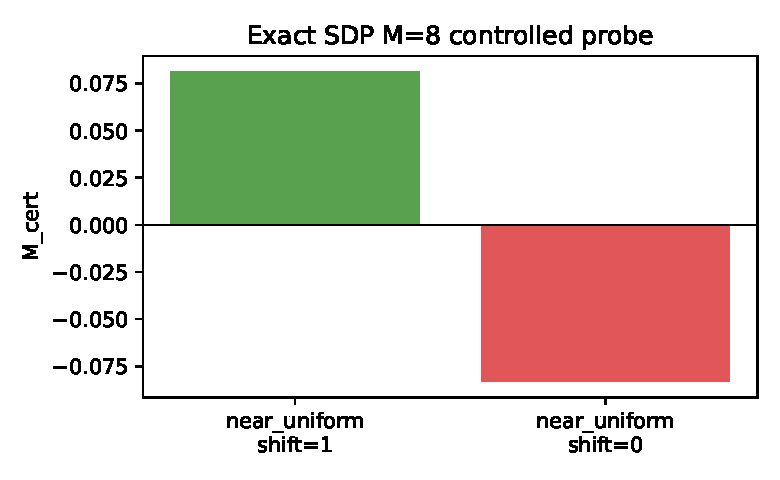
\includegraphics[width=\columnwidth]{paper_data/figures/exact_sdp_m8_probe.pdf}
\caption{\label{fig:m8-probe}Controlled SDP calculations for selected \(M=8\) finite instances. One solved instance has positive certificate margin and one comparable solved instance is negative, illustrating nonemptiness and instance dependence.}
\end{figure}



\subsection{Weighted resource sensitivity}

The weighted sensitivity analysis varies \(w_A/w_L\), \(w_Q/w_L\), and \(w_D/w_L\), with small fixed \(w_M/w_L\) and \(w_G/w_L\) diagnostics. Only \(1.90\%\) of weighted rows in the conservative default sensitivity scan have \(M_{\rm res}^{(w)}>0\), whereas the favorable-regime sweep has a weighted-positive fraction of \(0.347\). The default scan therefore represents conservative behavior, while the favorable-regime sweep maps structured low-overhead regions.

\begin{figure}[tbp]

\includegraphics[width=\columnwidth]{paper_data/figures/weighted_resource_sensitivity_heatmap.pdf}
\caption{\label{fig:weighted-sensitivity}Weighted-resource sensitivity heatmap for the default benchmark. The color gives the empirical positive-margin fraction under \(M_{\rm res}^{(w)}\) over the finite sampled rows. Positive regions persist for low modeled overheads but shrink as ancilla, QEC, or depth weights increase.}
\end{figure}

\subsection{QEC and MAP layers}

The QEC reliability analysis uses repetition-code, stabilizer-code, and depth-sensitive toy/proxy models. These models show how \(q_L\) changes the reported lower-bound proxy \((1-q_L)P_{\rm group}+q_LP_{\rm fallback}\), while the benchmark margins quantify the resulting resource efficiency. MAP supplies the posterior decision rule after the probabilistic decoder and fallback model.

\subsection{Four-symbol sanity check}

The angle-defined four-symbol construction provides a notation-level sanity check. It illustrates priors, Huffman lengths, a two-group partition, and the formula for \(P_{\rm full}\) in a transparent two-dimensional setting. The multi-\(M\) benchmark and scaling tests use the support-constrained payload rule.


\section{Discussion}

The proposed construction is a finite-resource probabilistic decoding framework in which Huffman lengths define support budgets and all states are decoded probabilistically from a common ambient Hilbert space. The group ancilla improves distinguishability by rendering inter-group alternatives orthogonal, while QEC improves reliability under the effective logical-failure model. Their resource value is determined by the normalized margin.

The ambiguity quantities \(\mathcal A_{\mathrm{Huff}}\) and \(\mathcal A_i\) show where source-weighted nonorthogonality enters the support-shaped ensemble. The transfer quantity \(\mathcal A_{\mathrm{sep}}\) and the grouping criterion \(J_{\mathrm{grp}}\) show how the group label changes the conditional discrimination tasks. The margin quantities \(M_{\rm res}\), \(M_{\rm cert}\), and \(\tau_{\mathrm{OH}}\) test whether the success gain pays for the extra resources, with success determined by the POVM/SDP decoder.

The SDP-certified condition directly compares a grouped primal lower certificate with a fixed-length dual upper certificate. Once the ensembles, resource accounting convention, and feasible SDP certificates are fixed, a positive normalized certificate gap gives a verifiable sufficient condition for strict resource advantage.

In the effective QEC model, smaller $q_L$ moves the success lower bound toward $P_{\mathrm{group}}$, while the same code contributes $C_{\mathrm{QEC}}$ to the denominator. The resource inequality captures this reliability--redundancy trade-off.

The three baselines serve different roles. The fixed-length global POVM baseline measures the combined effect of source-dependent support budgeting and grouping. The grouped no-QEC baseline isolates the ancilla contribution from physical redundancy. The QEC-assisted baseline measures the reliability gain after resource normalization.

The construction works with a finite source alphabet, finite supports, and explicitly counted ancilla and redundancy costs. Within each head-to-head certificate comparison, the ambient representation and state-construction convention are fixed. Comparisons in which the ambient dimension itself changes require an augmented cost model. The resulting scalar resource metric makes every certified gain appear as either higher success probability or lower modeled cost and supports finite-regime identification.

The conservative benchmark yields predominantly nonpositive margins under default overhead accounting. Within the deliberately sampled design space, the favorable-regime sweep identifies structured low-overhead, high-support-saving regions. Numerically verified SDP certificates validate selected finite instances where the SDP dimension is tractable. Together, these results establish a regime-identification and certification framework.

The scalar resource cost is convention dependent and represents group-label, redundancy, depth, measurement, and gate costs through declared proxy weights. The favorable-regime fractions summarize a finite designed sample. Numerical SDP certification scales poorly with alphabet and Hilbert-space dimension, and the effective $q_L$ layer abstracts architecture-specific fault-tolerant circuitry. A positive certificate applies to the specified ensembles and accounting convention; a failed certificate leaves the ordering unresolved.

The positive SDP-certified cases show that explicit support-driven ensembles can satisfy the finite-instance sufficient condition.

Hardware-native POVMs, calibrated fault-tolerant recovery, variable-depth state preparation, and device-level throughput require a more detailed architecture and resource-overhead model~\cite{fowler2012surface,terhal2015quantum,campbell2017roads}. The present POVM/SDP layer provides an optimal discrimination benchmark, and the logical-failure curves provide finite-resource reliability diagnostics. Architecture-specific refinements would change the cost model while preserving the resource test in Eq.~\eqref{eq:resource_advantage_condition}.

\section{Conclusion}

We introduced a quantum-Huffman-inspired finite-resource probabilistic source-decoding framework. Classical Huffman lengths define support-budget parameters in a common Hilbert space. The resulting states form a source-shaped ensemble whose ambiguity is summarized by \(\mathcal A_{\mathrm{Huff}}\) and \(\mathcal A_i\). The group ancilla removes inter-group ambiguity from the conditional POVM tasks, measured by \(\mathcal A_{\mathrm{sep}}\). The criterion \(J_{\mathrm{grp}}(\mathcal G)\) balances intra-group ambiguity, worst-case overlap, and label overhead. QEC and MAP enter as reliability and posterior layers.

The resource side is expressed through \(M_{\rm res}\), \(M_{\rm cert}\), and \(\tau_{\mathrm{OH}}\). These diagnostics state when a success or reliability gain becomes a resource-normalized advantage under the chosen accounting convention. The bounded-overlap theorem provides an analytic design criterion, and the SDP-certified theorem provides finite-instance certification from feasible primal and dual objects. The numerical diagnostics quantify the trade-off between reliability gain and modeled overhead.

The default benchmark yields predominantly nonpositive margins, whereas the favorable-regime sweep identifies structured low-overhead, high-support-saving regions and finite-instance SDP certificates verify selected positive \(M=4\) and \(M=8\) cases. These cases demonstrate that the proposed support-budget and group-conditioning mechanism can meet the resource inequalities in concrete finite regimes. Future work can replace each modular layer independently: hardware-native state preparation and conditional POVMs, architecture-calibrated logical channels and costs, and larger-scale certified optimization.

\appendix
\setcounter{theorem}{0}
\setcounter{figure}{0}
\setcounter{table}{0}
\renewcommand{\thetheorem}{\Alph{section}\arabic{theorem}}
\renewcommand{\thefigure}{\Alph{section}\arabic{figure}}
\renewcommand{\thetable}{\Alph{section}\arabic{table}}
\renewcommand{\theHfigure}{\Alph{section}.\arabic{figure}}
\renewcommand{\theHtable}{\Alph{section}.\arabic{table}}

\section{Gradients for Amplitude--Phase Overlap Optimization}
\label{app:gradients}

This appendix records the elementary gradients used by numerical overlap optimization. The main framework depends on the resulting overlap structure of the ensemble and admits different continuous optimization algorithms.

For
\begin{equation}
    z_{ij}=\braket{\Phi_i|\Phi_j}
    =
    \sum_x a_{i,x}a_{j,x}
    e^{i(\theta_{j,x}-\theta_{i,x})},
\end{equation}
the squared overlap is $G_{ij}=|z_{ij}|^2$. The phase derivative is
\begin{align}
    \frac{\partial G_{ij}}{\partial \theta_{i,y}}
    &=
    2\mathrm{Re}\left[
    -i a_{i,y}a_{j,y}
    e^{i(\theta_{j,y}-\theta_{i,y})}
    z_{ij}^{*}
    \right].
    \label{eq:phase_gradient}
\end{align}
The amplitude derivative is
\begin{align}
    \frac{\partial G_{ij}}{\partial a_{i,y}}
    &=
    2\mathrm{Re}\left[
    a_{j,y}e^{i(\theta_{j,y}-\theta_{i,y})}
    z_{ij}^{*}
    \right].
    \label{eq:amplitude_gradient}
\end{align}
For the weighted objective
\begin{equation}
    \mathcal{O}_{\mathrm{ov}}
    =
    \sum_{i<j}p_ip_j|\braket{\Phi_i|\Phi_j}|^2,
\end{equation}
the constrained amplitude stationarity condition under
$\sum_xa_{i,x}^2=1$ is
\begin{equation}
    \frac{\partial \mathcal{O}_{\mathrm{ov}}}{\partial a_{i,y}}
    +
    2\lambda_i a_{i,y}
    =
    0.
    \label{eq:lagrange_stationary}
\end{equation}
Using Eq.~\eqref{eq:amplitude_gradient}, this becomes
\begin{equation}
    \sum_{j\neq i} p_ip_j 2\mathrm{Re}\left[
    a_{j,y}e^{i(\theta_{j,y}-\theta_{i,y})}
    z_{ij}^{*}
    \right]
    +
    2\lambda_i a_{i,y}
    =
    0.
    \label{eq:amplitude_optimality}
\end{equation}

\section{SDP Validation Against the Helstrom Bound}
\label{app:sdp_validation}

The numerical SDP implementation was validated by comparing two-state SDP solutions against the analytic Helstrom formula. Twenty random pairs of pure states in dimension four were generated with random priors. The maximum absolute difference between the SDP value and the Helstrom value was approximately
\begin{equation}
    3.14\times10^{-9},
\end{equation}
well below the numerical tolerance used in the simulations. The validation data are stored in the Supplemental Material as \texttt{data/sdp\_helstrom\_validation.csv}.

\section{QEC Syndrome Model and SDP Details}
\label{app:qec_sdp_details}

\subsection{QEC syndrome model and logical-failure bound}
\label{app:qec_syndrome}

This appendix records the standard syndrome-level details underlying the effective logical-failure probability used in the main text. These details support the reliability layer of the framework.

Let $P_C=V_{\mathrm{QEC}}V_{\mathrm{QEC}}^\dagger$ denote the projector onto the code subspace. A set of errors $\{E_a\}$ is correctable if and only if
\begin{equation}
    P_C E_a^\dagger E_b P_C
    =
    \alpha_{ab}P_C
\end{equation}
for some Hermitian matrix $\alpha_{ab}$. This condition means that the syndrome can reveal which error occurred without revealing the encoded logical information.

For a stabilizer code with generators
\begin{equation}
    \mathcal{S}=\langle S_1,S_2,\ldots,S_m\rangle,
\end{equation}
a Pauli error $E_a$ determines a syndrome $s(a)$ through the commutation signs between $E_a$ and the generators. The corresponding syndrome projector is
\begin{equation}
    \Pi_s
    =
    \prod_{k=1}^{m}
    \frac{I+(-1)^{s_k}S_k}{2}.
\end{equation}
For a noisy state $\rho_i^{\mathrm{noisy}}$, the syndrome probability is
\begin{equation}
    P(s|i)
    =
    \mathrm{Tr}\left(\Pi_s\rho_i^{\mathrm{noisy}}\right).
\end{equation}
For a Pauli channel
\begin{equation}
    \mathcal{E}(\rho)=\sum_a q_aE_a\rho E_a^\dagger,
\end{equation}
this reduces to
\begin{equation}
    P(s|i)
    =
    \sum_{a:s(a)=s}q_a.
\end{equation}
Thus, in the ideal stabilizer-code abstraction under Pauli noise, the syndrome statistics depend on the physical error distribution but not on the logical source symbol.

For each syndrome $s$, let $C_s$ be a chosen correction operator, typically the inverse of the most likely error compatible with $s$. The recovery operation can be written as
\begin{equation}
    \mathcal{R}(\rho)
    =
    \sum_s
    C_s\Pi_s\rho\Pi_s C_s^\dagger .
\end{equation}
The correctable error set is
\begin{equation}
    \mathcal{A}_{\mathrm{corr}}
    =
    \{a:C_{s(a)}E_aP_C=P_C\}.
\end{equation}
The logical correction and failure probabilities are
\begin{equation}
    P_{\mathrm{corr}}
    =
    \sum_{a\in\mathcal{A}_{\mathrm{corr}}}q_a,
    \qquad
    q_L
    =
    1-P_{\mathrm{corr}}.
\end{equation}
For an $[[n,k,d]]$ stabilizer-code reliability proxy with independent physical error probability $p$ and $t=\lfloor(d-1)/2\rfloor$, assume independent occurrences of a specified physical-error family and correction of every error in that family with weight at most $t$. For this error family, the bound used in the main text is
\begin{equation}
    P_{\mathrm{corr}}
    \geq
    \sum_{w=0}^{t}
    \binom{n}{w}p^w(1-p)^{n-w}.
\end{equation}

\subsection{Primal POVM SDP}

For an ensemble $\{p_i,\rho_i\}_{i=1}^M$, minimum-error quantum-state discrimination is written as the POVM semidefinite program
\begin{align}
    P_{\mathrm{opt}}
    =
    \max_{\{E_i\}}
    &\sum_{i=1}^M p_i\mathrm{Tr}(E_i\rho_i)
    \label{eq:appendix_primal_sdp}\\
    \mathrm{subject\ to}\quad
    &E_i\succeq0,\qquad i=1,\ldots,M,\nonumber\\
    &\sum_{i=1}^M E_i=I.\nonumber
\end{align}
The variables $E_i$ are positive semidefinite measurement operators. The normalization constraint makes $\{E_i\}$ a POVM on the support Hilbert space used by the encoder.

\subsection{Lagrangian and dual problem}

Introducing a Hermitian dual variable $Y$ for the equality constraint $\sum_i E_i=I$, the Lagrangian is
\begin{equation}
    \mathcal{L}(\{E_i\},Y)
    =
    \sum_i p_i\mathrm{Tr}(E_i\rho_i)
    +
    \mathrm{Tr}\left[
    Y\left(I-\sum_iE_i\right)
    \right].
\end{equation}
Equivalently,
\begin{equation}
    \mathcal{L}(\{E_i\},Y)
    =
    \mathrm{Tr}(Y)
    +
    \sum_i
    \mathrm{Tr}\left[
    E_i(p_i\rho_i-Y)
    \right].
\end{equation}
The supremum over $E_i\succeq0$ is finite only if
\begin{equation}
    Y\succeq p_i\rho_i,\qquad i=1,\ldots,M.
\end{equation}
Thus the dual SDP is
\begin{align}
    D_{\mathrm{opt}}
    =
    \min_Y\quad
    &\mathrm{Tr}(Y)
    \label{eq:appendix_dual_sdp}\\
    \mathrm{subject\ to}\quad
    &Y\succeq p_i\rho_i,\qquad i=1,\ldots,M.\nonumber
\end{align}

\subsection{KKT conditions}

The Karush--Kuhn--Tucker conditions consist of primal feasibility,
\begin{equation}
    E_i\succeq0,\qquad \sum_iE_i=I,
\end{equation}
dual feasibility,
\begin{equation}
    Y\succeq p_i\rho_i,\qquad i=1,\ldots,M,
\end{equation}
and complementary slackness,
\begin{equation}
    (Y-p_i\rho_i)E_i=0,\qquad i=1,\ldots,M.
\end{equation}
Under Slater conditions, strong duality holds and
\begin{equation}
    P_{\mathrm{opt}}=D_{\mathrm{opt}}.
\end{equation}
These conditions are useful for interpreting the SDP decoder: a measurement effect can have support only on the subspace where the corresponding dual inequality is tight.

\subsection{Group-conditioned SDP}

For group $G_g$, let $q_i^{(g)}=p_i/p_g$ denote the conditional prior for $i\in G_g$, where $p_g=\sum_{i\in G_g}p_i$. The group-conditioned discrimination problem is
\begin{align}
    P_{\mathrm{opt}}^{(g)}
    =
    \max_{\{E_i^{(g)}\}}
    &\sum_{i\in G_g}q_i^{(g)}
    \mathrm{Tr}\left(E_i^{(g)}\rho_i^{(g)}\right)
    \label{eq:appendix_group_sdp}\\
    \mathrm{subject\ to}\quad
    &E_i^{(g)}\succeq0,\qquad i\in G_g,\nonumber\\
    &\sum_{i\in G_g}E_i^{(g)}=I_g.\nonumber
\end{align}
The ideal group-conditioned success probability is then
\begin{equation}
    P_{\mathrm{group}}=\sum_gp_gP_{\mathrm{opt}}^{(g)}.
\end{equation}
Group conditioning retains the POVM framework while replacing one large SDP over all symbols by several smaller SDPs for the conditional ensembles.

\FloatBarrier
\section{Additional Randomized Numerical Statistics}

The randomized statistics in this appendix are computed from \texttt{randomized\_ensemble\_validation.csv}. They provide robustness checks showing whether the mechanisms predicted by the theoretical bounds persist across randomized ensembles.

The randomized protocol uses alphabet sizes \(M\in\{4,8,16,32\}\). For each trial, source probabilities are drawn from a Dirichlet distribution and payload states are sampled as normalized complex Gaussian pure states in dimension four. Numerical SDP baselines are used for \(M=4\) and for selected low-dimensional \(M=8\) diagnostic rows where the solver records a solved status; larger scalable rows use the pretty-good measurement and the CSV records the approximation through the corresponding baseline-type columns. These randomized statistics provide robustness diagnostics. The grouping strategies are random grouping, probability-aware grouping, and overlap-aware grouping. Recorded metrics include \(P_{\mathrm{base,opt}}\), \(P_{\mathrm{group}}\), \(P_{\mathrm{group}}-P_{\mathrm{base,opt}}\), \(P_{\mathrm{full}}\), \(\eta\), and the overlap-ratio diagnostic \(\epsilon_{\mathrm{global}}/\epsilon_{\mathrm{in}}\).

The three grouping rules separate different sources of improvement. Random grouping provides a distribution-free reference. Probability-aware grouping distributes high-priority symbols across groups. Overlap-aware grouping uses the sampled Gram matrix and greedily reduces the largest within-group squared overlap. For each trial the same ensemble is evaluated under all three strategies, so the reported differences isolate the grouping choice with the source distribution and payload states fixed.

The randomized QEC-assisted quantities use the same effective lower bound as the main text,
\begin{equation}
    P_{\mathrm{full}}\geq(1-q_L)P_{\mathrm{group}}+q_LP_{\mathrm{fallback}},
\end{equation}
with the right-hand side reported as the numerical lower-bound proxy, and
\begin{equation}
    \eta=\frac{P_{\mathrm{full}}}{\bar L+C_A+C_{\mathrm{QEC}}}.
\end{equation}
Thus the randomized tables test whether grouping gains persist after the reliability model and resource normalization are applied.

\begin{table}[!htb]
\caption{\label{tab:appendix_randomized_protocol}Randomized ensemble validation protocol.}
\scriptsize
\begin{ruledtabular}
\begin{tabular}{ll}
Item & Setting\\
\hline
Alphabet sizes & \(M\in\{4,8,16,32\}\)\\
Source priors & Dirichlet-distributed probability vectors\\
Payload states & normalized complex Gaussian pure states\\
Hilbert dimension & \(d=4\)\\
Small diagnostic baseline & SDP: \(M=4\); selected \(M=8\)\\
Scalable baseline & PGM for larger rows\\
Grouping rules & random, probability-aware, overlap-aware\\
Success metrics & \(P_{\mathrm{base,opt}}\), \(P_{\mathrm{group}}\), \(P_{\mathrm{full}}\)\\
Resource/overlap metrics & \(\eta\), grouping gain, overlap ratio\\
\end{tabular}
\end{ruledtabular}
\end{table}

\begin{table}[!htb]
\caption{\label{tab:appendix_gain_stats}Grouping gain statistics by alphabet size and strategy. Statistics are computed over randomized ensembles using one row per trial and strategy.}
\begin{ruledtabular}
\begin{tabular}{lccc}
$M$ & Strategy & Mean $\pm$ std. & Range\\
\hline
$4$ & overlap-aware & $0.1090\pm0.0545$ & $0.0377$--$0.2575$\\
$4$ & probability-aware & $0.0941\pm0.0515$ & $0.0037$--$0.2575$\\
$4$ & random & $0.0895\pm0.0489$ & $0.0117$--$0.1985$\\
$8$ & overlap-aware & $0.2100\pm0.0523$ & $0.0860$--$0.3303$\\
$8$ & probability-aware & $0.1798\pm0.0573$ & $0.0484$--$0.3548$\\
$8$ & random & $0.1765\pm0.0536$ & $0.0660$--$0.3059$\\
$16$ & overlap-aware & $0.5401\pm0.0482$ & $0.4170$--$0.6105$\\
$16$ & probability-aware & $0.4773\pm0.0473$ & $0.3496$--$0.5610$\\
$16$ & random & $0.4708\pm0.0444$ & $0.3643$--$0.5561$\\
$32$ & overlap-aware & $0.6090\pm0.0221$ & $0.5654$--$0.6470$\\
$32$ & probability-aware & $0.5429\pm0.0343$ & $0.4635$--$0.6118$\\
$32$ & random & $0.5219\pm0.0267$ & $0.4601$--$0.5717$\\
\end{tabular}
\end{ruledtabular}
\end{table}

\begin{table}[!htb]
\caption{\label{tab:appendix_reliability_eta_stats}QEC-assisted success and resource-efficiency statistics for the randomized ensembles.}
\begin{ruledtabular}
\begin{tabular}{lccc}
$p$ & Strategy & $P_{\mathrm{full}}$ & $\eta$\\
\hline
$0.02$ & overlap-aware & $0.9172\pm0.0558$ & $0.08293\pm0.01556$\\
$0.02$ & probability-aware & $0.8771\pm0.0741$ & $0.07961\pm0.01700$\\
$0.02$ & random & $0.8691\pm0.0796$ & $0.07894\pm0.01730$\\
$0.05$ & overlap-aware & $0.8946\pm0.0573$ & $0.08093\pm0.01550$\\
$0.05$ & probability-aware & $0.8588\pm0.0770$ & $0.07800\pm0.01710$\\
$0.05$ & random & $0.8483\pm0.0804$ & $0.07709\pm0.01718$\\
$0.10$ & overlap-aware & $0.8295\pm0.0624$ & $0.07518\pm0.01535$\\
$0.10$ & probability-aware & $0.8059\pm0.0868$ & $0.07337\pm0.01744$\\
$0.10$ & random & $0.7883\pm0.0832$ & $0.07175\pm0.01683$\\
\end{tabular}
\end{ruledtabular}
\end{table}

\FloatBarrier
\section{Additional Phase Diagrams}
\label{app:additional_phase}

This appendix reports additional resource-advantage diagnostics generated from the same margin used in the main text,
\begin{equation}
    M_{\rm res}
    =
    P_{\mathrm{full}}
    -
    P_{\mathrm{base,opt}}
    \left(1+\frac{\Delta C}{C_{\mathrm{base}}}\right),
\end{equation}
where
\begin{equation}
    P_{\mathrm{full}}
    \geq
    (1-q_L)P_{\mathrm{group}}+q_LP_{\mathrm{fallback}}.
\end{equation}
The plots evaluate the right-hand side as the reported lower-bound proxy. They are parameter-regime diagnostics for the resource margin. The boundary and threshold views visualize the model-specific finite-resource overhead tolerance \(\tau_{\mathrm{OH}}\) of Eq.~\eqref{eq:overhead_tolerance}.

\begin{figure*}[t]
\centering
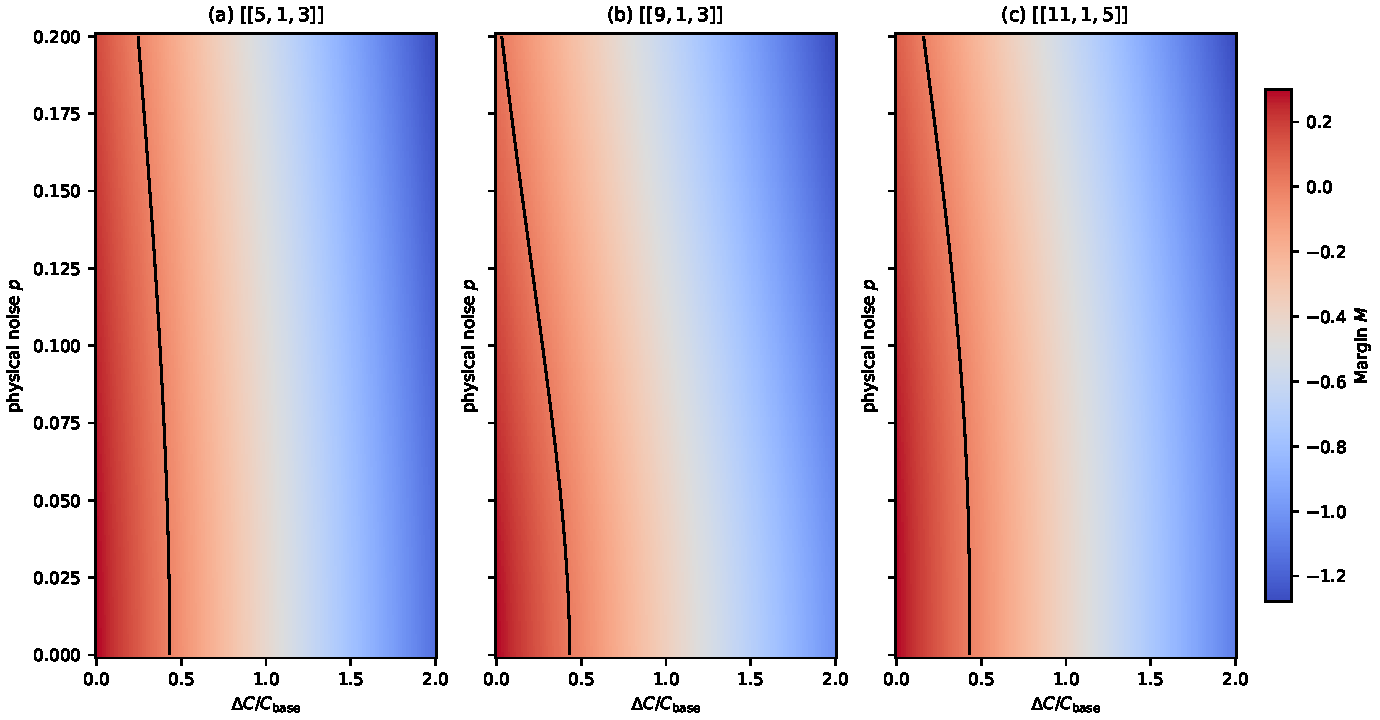
\includegraphics[width=\textwidth]{paper_data/figures/appendix_e1_phase_triptych.pdf}
\caption{\label{fig:appendix-code-phase}Additional enhanced resource-advantage phase diagrams for (a) the $[[5,1,3]]$ code model, (b) the $[[9,1,3]]$ code model, and (c) the $[[11,1,5]]$ code model. All panels evaluate \(P_{\mathrm{full}}\) by the lower-bound proxy above and use the margin \(M_{\rm res}=P_{\mathrm{full}}-P_{\mathrm{base,opt}}(1+\Delta C/C_{\mathrm{base}})\); positive values indicate regimes where the modeled success gain compensates the modeled overhead.}
\vspace{0.3ex}
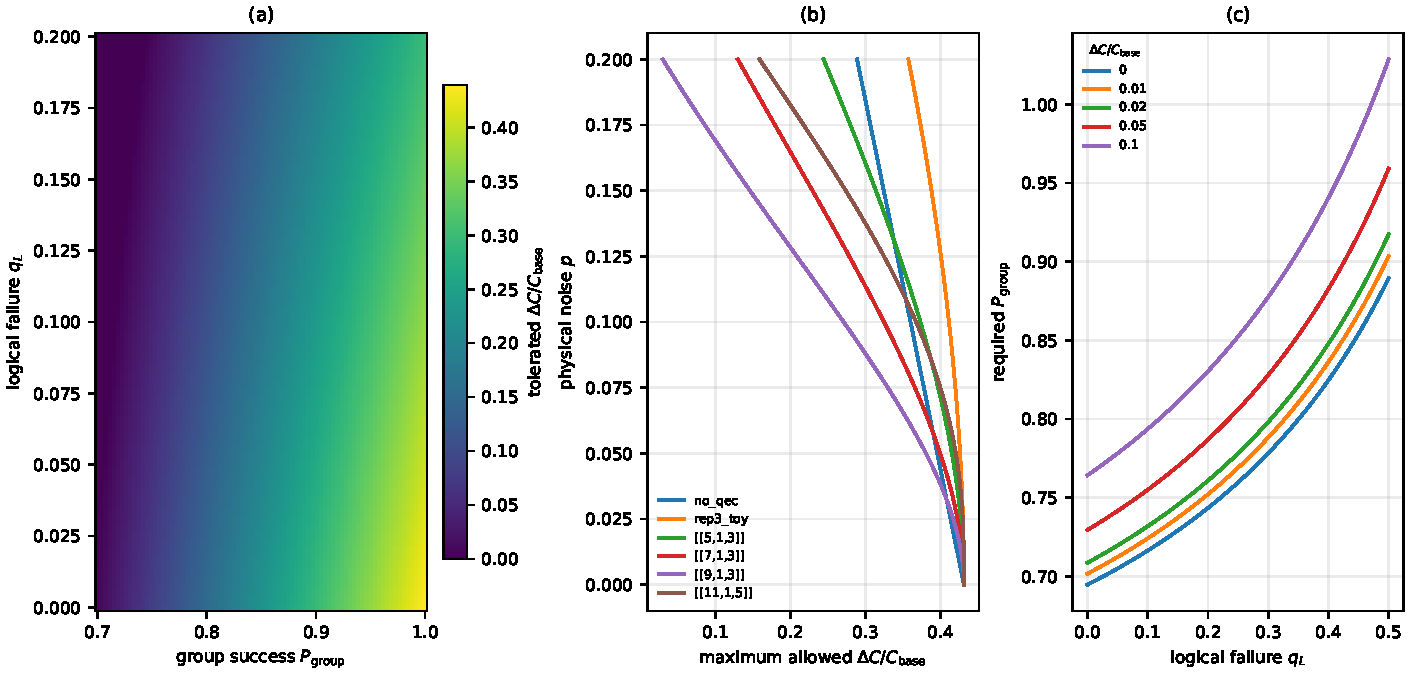
\includegraphics[width=\textwidth]{paper_data/figures/appendix_e2_resource_diagnostics.pdf}
\caption{\label{fig:appendix-grouping-quality}\label{fig:phase-boundary}\label{fig:required-threshold}Additional resource-margin and overhead-tolerance diagnostics. (a) Tolerated overhead as a function of group success and logical failure. (b) Boundary comparison by code model. (c) Required group success threshold for representative overhead ratios.}
\end{figure*}

\FloatBarrier
\section{Complexity Analysis}

The symbols \(\mathcal C_{\mathrm{global}}\) and \(\mathcal C_{\mathrm{group}}\) in this appendix denote computational-complexity proxies for SDP solution cost. They are distinct from the modeled resource costs \(C_{\mathrm{total}}\), \(C_A\), and \(C_{\mathrm{QEC}}\) used in Sec.~\ref{sec:resource_advantage}.

\subsection{Global POVM SDP complexity}

Let $M$ be the alphabet size and $d$ be the Hilbert-space dimension. The global POVM SDP uses $M$ positive semidefinite variables of size $d\times d$, so the decision-variable scale is $O(Md^2)$. A conservative interior-point scaling proxy is
\begin{equation}
    \mathcal C_{\mathrm{global}}\sim O(M^3d^6).
\end{equation}
This expression is a rough scaling proxy; first-order solvers and problem structure can change practical runtime substantially.

\subsection{Group-conditioned SDP complexity}

Let $m_g=|\mathcal G_g|$ be the size of group $g$. Solving the conditional SDPs separately gives the proxy
\begin{equation}
    \mathcal C_{\mathrm{group}}
    \sim
    \sum_g O(m_g^3d^6).
\end{equation}
If the groups are balanced, $m_g\approx M/G$, and therefore
\begin{equation}
    \mathcal C_{\mathrm{group}}
    \sim
    G\left(\frac{M}{G}\right)^3d^6
    =
    O\left(\frac{M^3d^6}{G^2}\right).
\end{equation}
Thus group conditioning can reduce the SDP scaling by roughly a factor $O(G^2)$, ignoring ancilla overhead, implementation constants, and solver details.

\subsection{Grouping algorithm complexity}

Computing the pairwise overlap matrix for $M$ states in dimension $d$ costs
\begin{equation}
    O(M^2d).
\end{equation}
The greedy overlap-aware grouping heuristic used in the randomized experiments costs approximately
\begin{equation}
    O(M^2G+M^2d).
\end{equation}
Grouping is combinatorial in general, but greedy polynomial-time heuristics are sufficient for numerical exploration and for diagnosing whether the theoretical grouping conditions can be favorable.

\subsection{Pretty-good measurement approximation}

For larger randomized ensembles, the numerical global SDP is replaced by the pretty-good measurement baseline. Define
\begin{equation}
    \Gamma=\sum_ip_i\rho_i.
\end{equation}
The PGM effects are standard in quantum detection and recovery analyses~\cite{hausladen1994pretty,eldar2001quantum,barnum2002reversing}
\begin{equation}
    E_i^{\mathrm{PGM}}
    =
    \Gamma^{-1/2}p_i\rho_i\Gamma^{-1/2},
\end{equation}
where the inverse is the Moore--Penrose inverse on the support of \(\Gamma\).
The approximate cost is dominated by matrix decompositions and multiplications, with scaling on the order of
\begin{equation}
    O(d^3+Md^3),
\end{equation}
or simply $O(Md^3)$ for fixed implementation constants. In this work, PGM is used as the scalable approximate baseline for larger randomized ensembles. Numerical SDP evidence is limited to \(M=4\) certificate statistics and selected solved \(M=8\) probes.

\subsection{Resource complexity}

The resource model used in the numerical experiments is
\begin{equation}
    C_{\mathrm{total}}=\bar L+C_A+C_{\mathrm{QEC}},
\end{equation}
with
\begin{equation}
    C_A=\lceil\log_2G\rceil,
\end{equation}
and, when a redundancy multiplier \(r\geq0\) and symbol-dependent logical support costs \(n_i\geq0\) are declared, one optional QEC-cost proxy is
\begin{equation}
    C_{\mathrm{QEC}}=\sum_ip_irn_i.
\end{equation}
The numerical studies state their chosen \(C_{\mathrm{QEC}}\) directly as a declared proxy. Increasing $G$ can improve grouping gain but also increases ancilla cost. Increasing the declared redundancy multiplier $r$ can reduce $q_L$ in the reliability proxy while increasing QEC cost. Therefore reliability gain and resource-normalized efficiency remain distinct metrics.

\FloatBarrier
\section{Supplementary Numerical Diagnostics}
\label{app:supplementary_diagnostics}
\setcounter{figure}{0}
\setcounter{table}{0}

This appendix presents supplementary diagnostics of support overlap, grouping, reliability, and finite-instance certification.

The communication-level diagnostics use the same finite ensemble as the discrimination experiments but insert a local noise channel before the approximate decoder. The plotted channel families include local depolarizing, amplitude-damping, and phase-damping noise. They test whether grouping remains useful when the prepared states are imperfect and whether the effective QEC proxy produces the expected reliability trend. These plots provide qualitative finite-resource diagnostics.

\begin{center}
\refstepcounter{table}\label{tab:appendix_diagnostic_roles}
\scriptsize
\textbf{TABLE~\thetable.} Roles of the supplementary numerical diagnostics.\\[0.5ex]
\begin{ruledtabular}
\begin{tabular}{ll}
Diagnostic family & Role in the paper\\
\hline
Overlap-ratio & grouping separates ambiguous pairs\\
Zipf support & support-budget saving under source skew\\
Logical failure & effective \(q_L(p)\) reliability proxies\\
Communication & robustness under local noise\\
Randomized boxplots & gains across sampled ensembles\\
Support-driven & Huffman support consistency\\
SDP certificates & instance certificate margins\\
Efficiency & reliability/overhead trade-off\\
\end{tabular}
\end{ruledtabular}
\end{center}

\newcommand{\appdiagfig}[3]{%
\par\medskip
\noindent\begin{minipage}{\columnwidth}
\centering
\refstepcounter{figure}\label{#1}%
\includegraphics[width=0.98\columnwidth,height=0.30\textheight,keepaspectratio]{#2}\par\vspace{0.5ex}
\footnotesize\raggedright
\textbf{FIG.~\thefigure.} #3
\end{minipage}
\par\medskip
}

\paragraph*{Overlap and support diagnostics.}
These figures provide design diagnostics of bounded overlap and the support-budget layer.

\appdiagfig{fig:grouping-ratio}{paper_data/figures/grouping_gain_vs_overlap_ratio.pdf}{Overlap-ratio diagnostic for the bounded-overlap comparison. Larger $\epsilon_{\mathrm{global}}/\epsilon_{\mathrm{in}}$ indicates that highly overlapping states are placed in different groups, increasing conditional distinguishability.}

\appdiagfig{fig:zipf-gain}{paper_data/figures/zipf_compression_gain.pdf}{Average support-budget gain \(G_{\mathrm{comp}}=n_{\mathrm{fix}}-\bar L\) induced by Huffman-length allocation. The gain becomes small near a uniform source and grows as the source distribution becomes more skewed in the sampled family.}

\appdiagfig{fig:app-support-overlap}{paper_data/figures/support_overlap_vs_A_Huff.pdf}{Support-overlap diagnostic for the benchmark and favorable-regime sweep. The normalized overlap ratio \(R_{\rm sup}\) is a design variable, and the plot reports its empirical relation to \(\mathcal A_{\rm Huff}\).}

\paragraph*{Reliability and communication diagnostics.}
These proxy/noisy-channel figures test robustness trends in the effective reliability layer.

\appdiagfig{fig:qec-logical}{paper_data/figures/qec_logical_failure_vs_noise.pdf}{Logical failure probability under the proxy \(q_L\le 1-\sum_{w=0}^{t}\binom{n}{w}p^w(1-p)^{n-w}\). The curve labeled \texttt{rep3\_toy} is a three-qubit repetition-style toy model for bit-flip logical failure.}

\appdiagfig{fig:communication-grouping-advantage}{paper_data/figures/communication_grouping_advantage.pdf}{Grouping advantage under communication-level noisy transmission. The plotted gap $P_{\mathrm{success,group}}-P_{\mathrm{success,no\ group}}$ shows whether the group ancilla remains useful after local noise is applied.}

\paragraph*{Randomized and scalable diagnostics.}
These figures summarize approximate or randomized ensemble robustness tests; SDP certificate evidence is reported separately.

\appdiagfig{fig:randomized-strategy}{paper_data/figures/randomized_grouping_strategy_comparison.pdf}{Comparison of grouping strategies. The plot reports the statistical advantage of overlap-aware grouping across the sampled ensembles.}

\appdiagfig{fig:app-randomized-eta}{paper_data/figures/randomized_eta_boxplot.pdf}{Distribution of resource-normalized efficiency over randomized ensembles, using \(\eta=P_{\mathrm{full}}/C_{\mathrm{total}}\) with \(C_{\mathrm{total}}=\bar L+C_A+C_{\mathrm{QEC}}\).}

\paragraph*{Support-driven and certificate diagnostics.}
These figures connect the support-allocation construction to finite-instance certificate behavior and distinguish SDP certificates from approximate scalable diagnostics.

\appdiagfig{fig:app-support-budget}{paper_data/figures/support_budget_validation.pdf}{Support-budget validation for a Huffman-allocated four-symbol source. Each support size satisfies \(|S_i|\le 2^{n_{\max}-l_i}\), and the total occupied support is within the ambient dimension.}

\appdiagfig{fig:app-ambiguity-transfer}{paper_data/figures/ambiguity_transfer_by_grouping.pdf}{Ambiguity transfer for three groupings of the four-symbol support-driven ensemble. The group label removes \(\mathcal A_{\mathrm{sep}}\) from the conditional POVM tasks and leaves \(\mathcal A_{\mathrm{in}}\).}

Figure~\ref{fig:app-sdp-cert} separates support feasibility from certified advantage for the initial four-symbol support-driven cases.

\appdiagfig{fig:app-sdp-cert}{paper_data/figures/sdp_certificate_margin.pdf}{SDP certificate margins for the four-symbol support-driven cases. The certificate is instance dependent, and a negative margin leaves this sufficient test inconclusive.}

\appdiagfig{fig:app-best-positive-regenerated}{paper_data/figures/best_positive_certificate_instance.pdf}{Positive finite-instance SDP certificate with the largest margin in the \(M=4\) sample, shown as an instance-level certificate illustration.}

\appdiagfig{fig:app-negative-regenerated}{paper_data/figures/representative_negative_certificate_instance.pdf}{Representative negative finite-instance SDP certificate. The negative margin leaves this sufficient test inconclusive for the instance.}

\FloatBarrier
\section*{Data availability}

The data and code supporting the findings of this study are provided in the Supplemental Material~\cite{supplemental_material} and in the accompanying reproducibility package. The package contains scripts to reproduce Huffman support allocation, support-constrained payload generation, group-conditioned SDP/PGM decoding, QEC reliability proxies, certificate search, resource-sensitivity diagnostics, favorable-regime analysis, support-overlap analysis, and all figures used in the manuscript.

\bibliographystyle{apsrev4-2}
\bibliography{references}

\end{document}
% ****** End of file main.tex ******
